\documentclass[11pt, a4paper]{article}

\usepackage[utf8]{inputenc}
\usepackage{amsfonts}
\usepackage{amsmath}
\usepackage{hyperref}
\usepackage{graphicx}
\usepackage[frenchb]{babel}
\usepackage[left=3cm, right=3cm]{geometry}

% Headers & footers
\usepackage{fancyhdr}
\pagestyle{fancyplain}
\fancyhead[LE]{\fancyplain{}{}}
\fancyhead[CE]{\fancyplain{}{}}
\fancyhead[RE]{\fancyplain{}{\bfseries\leftmark}}
\fancyhead[LO]{\fancyplain{}{\bfseries\rightmark}}
\fancyhead[CO]{\fancyplain{}{}}
\fancyhead[RO]{\fancyplain{}{}}
\fancyfoot[LE]{\fancyplain{}{}}
\fancyfoot[CE]{\fancyplain{}{}}
\fancyfoot[RE]{\fancyplain{}{}}
\fancyfoot[LO]{\fancyplain{}{}}
\fancyfoot[CO]{\fancyplain{}{\bfseries\thepage}}
\fancyfoot[RO]{\fancyplain{}{}}
% \renewcommand{\footrulewidth}{0.4pt}

\begin{document}

\title{Modélisation mathématique d'une cellule dans une population par des
réseaux booléens}
\author{Turpin Pierre, \\
    Étudiant au département informatique de l'INSA de Lyon, \\
    Maitre de stage : Samuel Bernard, \\
    \texttt{pierre.turpin@insa-lyon.fr}
}
\date{\today}

% Informations personnelles (nom, mail, maitre de stage)

\maketitle \newpage

% Résumé (150 mots max)
\begin{abstract}
    Les réseaux booléens sont des automates cellulaires permettant de simuler
    des applications et des machines à état plus ou moins complexe tout en
    gardant une approche discrète du problème.

    Ces réseaux sont utilisés pour modéliser et simuler des caractéristiques
    intracellulaires afin de reproduire au plus près possible les comportement
    de cellules en prolifération. La cellule en question est composée de
    plusieurs machines booléennes schématisant son évolution et ses choix au
    sein d'une population.

    Les réseaux booléens intracellulaires modélisent la survie ou la mort de la
    cellule, la progression dans le cycle cellulaire et l'horloge circadienne.

    Plusieurs cellules sont simulées dans un espace physique restreint et
    peuvent s'échanger des informations par contact. Cela lie les cellules
    entre elles et permet de simuler une population entière régit par des
    règles locales. % TODO parler des résultats

    On arrive alors à reproduire des mécanismes globaux tels que
    l'établissement d'une horloge circadienne globale ou encore la mort et la
    mutation des cellules.

    La prise en compte des mécanisme de décision cellulaire et de l'interaction
    entre cellules permet de reproduire finalement la dynamique d'une
    population de cellule en prolifération.
\end{abstract} \newpage

\tableofcontents \newpage

% Introduction (5 pages)
\section{Introduction}
L'utilisation des réseaux booléens permet de décrire des systèmes complexes
afin de modéliser plus facilement des dynamiques complexes. Ainsi il est possible de
tester et simuler ne très grand nombre de cas rapidement et efficacement grâce
à la taille réduite de l'espace des états possible du réseau \cite{greil2012}.
En effet, un réseau booléen est représenté par un ensemble d'états à valeur
dans $ {0, 1} $ ainsi qu'un ensemble de règles de transition dictant le
comportement de la machine. Chacun des éléments de l'état global du réseau est
représenté par un noeud. Les règles de transition sont alors symbolisées par
des arêtes entre les noeuds et correspondent à des interactions soit positive
(activatrices), soit inhibitrices. Pour simplifier la représentation des règles
de transition, celles-ci sont vu comme un ensemble de fonctions prenant l'état
courant du graphe et évaluant une réponse booléenne. Chaque noeud du réseau a sa
propre fonction de mise à jour. L'échelle temporelle des réseaux booléens est
discret. À chaque pas, l'ensemble des règles de transitions est appliqué d'une
certaine façon afin de mettre à jour la machine. Il existe différentes façons
d'appliquer ces règles, et ceci a une influence sur la dynamique et l'évolution
du réseau. Un postulat choisit, parmi l'ensemble des règles de mise à jour,
lesquelles seront utilisés. Si ce postulat est vrai pour tous les noeuds, alors les valeurs
d'état de tous les noeuds sont mises à jour. Si cette fonction n'est vrai que pour un
noeud, alors seul ce noeud est mis à jour. Il existe par exemple des
règles de mise à jour déterministes et d'autres stochastiques. Les solutions
utilisées seront présentées par la suite dans l'explication détaillée de chaque
machine utilisée. \\

D'un point de vue mathématique, on peut donc définir les réseaux booléens de
taille $N$ à l'instant $t$ de façon plus formelle : \\
Univers des états possibles : $ K = \{0, 1\} $ \\
Ensemble des noeuds du réseau : $ U_N = \{A_0, \dots, A_N\}$ \\
Ensemble des règles de mis à jour : $ F : K^N \rightarrow K $ \\
Ensemble des postulats en fonction du temps :
$ P : \mathbb{N} \rightarrow {\mbox{Vrai}, \mbox{Faux}} $ \\
Ensemble des états du réseau : $ E : \mathbb{N} \rightarrow K^N $ \\
Soit $i\in U_N$ un noeud du réseau. \\
Soit $E_i \in E, F_i \in F, P_i \in P$ respectivement l'état, la règle de mise
à jour et le postulat de choix du noeud d'indice $i$ défini. \\
La mis à jour du noeud $i$ :
$$
E_i(t + 1) =
\left\{\begin{array}{rl}
    F_i(E_0(t), \dots, E_N(t)) & \mbox{si $P_i(t)$} \\
    E_i(t) & \mbox{sinon}
\end{array}\right.
$$ \\
A chaque avancé au pas du réseau booléen, tous les noeuds sont mis à jour grâce
à leur règle et leur postulat. \\

Ces réseaux booléens sont utilisés pour simuler et tenter de voir le
comportement cellulaire d'abord à l'échelle intracellulaire puis à l'échelle
d'une population. Les cellules en contact peuvent communiquer entre elles. Ces
interactions extra cellulaires, par exemple par l'interm\'ediaire de cytokines, sont limitées dans le modèle
choisi. Chacune de ces voies de communication (entrées et sorties) correspond à une machine booléenne
utilisé en interne par une cellule et représente la dynamique d'une des
caractéristiques cellulaires. Dans le modèle utilisé, une cellule est composée
de quatre machines booléennes différentes qui sont présentées ci-dessous.

\subsection{Choix du destin cellulaire}
La première machine booléenne permet de savoir si la cellule survie ou si elle
meurt par apoptose ou par nécrose. Elle ne s'occupe uniquement de cet aspect et
ne gère pas d'autres composantes cellulaires. Elle possède deux entrées :
l'activation des noeuds \texttt{TNF} et \texttt{FAS} \cite{calzone2010}. Le
\texttt{TNF} correspond au facteur de nécrose tumorale et le \texttt{FAS} à la
protéine transmembranaire du même nom. Nous admettons que ces deux récepteurs,
une fois activés, sont les déclencheurs de la mort cellulaire par apoptose ou
par nécrose. On relèvera alors dans le réseau booléen utilisé le résultat de la
simulation par le test de trois noeuds : $NF\kappa B$, \texttt{ATP} et
\texttt{CASP3}. Le premier noeud $NF\kappa B$ correspond à la modélisation
booléenne de la présence de la protéine du même nom. Si ce noeud est activé,
alors on conclue à la survie de la cellule. Le second noeud \texttt{ATP}
correspond à la présence d'adénosine-triphosphate qui doit être nécessairement
produite et présente pour garantir la survie \cite{kroemer2007}. L'absence de
cette molécule et donc la désactivation du noeud \texttt{ATP} entraîne la mort
par nécrose de la cellule. Le dernier noeud, le \texttt{CASP3} correspond à la
protéine Caspase 3. Elle fait partie de la famille des protéines caspases et
joue donc un rôle central dans l'activation de la mort par apoptose de la
cellule \cite{porter1999}. La présence de cette protéine entraine la mort de la
cellule par apoptose. Ces réponses sont dites booléennes car on détermine
uniquement la présence ou non des protéines et non leur quantité. Le destin de
chaque cellule est déterminé en fonction des résultats de la machine booléenne.
Elle converge sur un seul choix, soit la survie, soit la mort par apoptose ou
par nécrose. Si plus d'un choix est fait, alors le destin cellulaire n'est pas
conclu et la machine booléenne continue et la cellule survie.

\subsection{Détermination de l'évolution du cycle cellulaire}
La deuxième machine booléenne utilisé en intracellulaire est celle indiquant
l'évolution du cycle cellulaire. Le modèle utilisé reprend des travaux sur des
réseaux du cycle d'une levure \cite{li2004}. En effet, ce modèle est bien connu
et la taille réduite du modèle ainsi que son déterminisme permet de connaître
tous les cas et tous les bassins d'attractions du modèle.  Il n'a qu'un seul
point d'entrée : la taille de la cellule. Cette entrée étant booléen, elle
correspond à la taille minimale de la cellule prise en compte. En effet, ce
noeud est placé en amont du réseau et son activation crée une activation en
cascade du réseau jusqu'à la convergence, d'après les résultats obtenus. La
sortie n'est pas booléenne puisqu'il s'agit d'essayer de déterminer la
progression de la cellule dans son cycle. À savoir $G1$, $S$, $G2$ ou $M$.
$G1$ correspond à la croissance de la cellule et à la duplication des éléments
cellulaires. $S$ est la synthèse de l'$ADN$. En $G2$, la cellule se prépare
pour la mitose. $M$ est la phase durant laquelle la cellule est en mitose.
D'après ces définitions il est alors possible de répondre et d'agir en
conséquence en fonction du résultat trouvé par la machine booléenne.

\subsection{Le choix entre différenciation et renouvellement}
La quatrième machine permet de faire le choix entre la différentiation de la
cellule ou son renouvellement lorsqu'elle est dans un état mitotique. Ce modèle
se base sur l'article \cite{palani2008}. Cette machine reproduit le système
simplifié de l'activation de la protéine \texttt{GATA-1} par la présence de
l'érythropoïétine (\texttt{EPO}). Cette dynamique simplifié représente cette
interaction comme une bascule à deux états bistables. Il n'y a qu'une seule
entrée dans ce réseau booléen. C'est celle qui indique la présence
d'\texttt{EPO} dans l'environnement de la cellule. Pour éviter que des petites
quantités de cette protéine soit prise en compte et que la bascule s'active, un
délai de taille variable doit être placé pour agir comme un filtre passe bas
sur le signal de la présence de la protéine.

\subsection{Horloge circadienne interne} \label{intro_clock}
La quatrième machine est une horloge booléenne symbolisant l'horloge
circadienne de la cellule \cite{akman2012}. Cette machine booléenne est composé
de seulement deux noeuds s'activant l'un après l'autre. L'un correspond à la
période du jour tandis que l'autre correspond à la période nocturne. Les deux
ne peuvent donc pas être actifs en même temps par définition. Cette machine a
une entrée représentant la présence de la lumière. Si la lumière est présente
pendant un certain délai prédéfini, alors elle provoque l'éveil de l'horloge et
le noeud correspondant au jour est mis à $1$ tandis que l'autre, la nuit, est
mis à $0$. Cette horloge étant binaire est trop simpliste pour modéliser une
véritable horloge circadienne agissant sur les cellules.
La cellule sera capable par contre de traiter l'information et d'approximer les
résultats souhaités. Il est toutefois possible d'avoir des horloges plus
complexes suivant d'autres types de modèles comme le modèle Neurospora à une et
deux boucles\cite{akman2008, leloup1999}, ou le modèle Arabidopsis à deux ou
trois boucles\cite{locke2005, locke2006}.

\subsection{Intégration dans une population}
L'ensemble de ces machines est inclus dans le modèle cellulaire. La cellule
possède elle-même un référentiel temporel absolu compté en heure dans le modèle
et cela oblige l'utilisation de nombres réels pour représenter le temps et la
durée. Les machines étant booléennes ne fonctionnent qu'avec des pas de temps
discrets. Un pas d'une machine correspond donc a une certaine quantité de temps
à définir. Il y a donc un facteur de mise à l'échelle du temps entre la cellule
et chacune des machines. Cela permet de pouvoir contrôler la rapidité de chaque
machine indépendamment pour que cela puisse correspondre et s'approcher au
mieux des résultats expérimentaux collectés et admis. La simulation d'une
cellule se fait par l'avancée de l'horloge interne de celle-ci.

Les machines intracellulaires sont alors automatiquement mis à jour et avance
d'un certain nombre de pas réglable par le facteur de temps. Avant chaque
avancée temporelle de la cellule, un modèle physique est appliqué prenant les
cellules comme des sphères viscoélastiques avec un noyau dur et un corps mou.
Les cellules qui sont alors en contact échangent certaines de leurs
informations intracellulaires. Ces échanges représentent des cytokines du
système de signalisation cellulaire.

Après la mise à jour cellulaire, les informations générales de la cellule sont
également modifiées grâce aux résultats obtenus de la part des différentes
machines interne au système.  Dans le modèle utilisé, des flags d'états
montrant différents statuts de la cellule sont utilisés pour gérer la
modification des informations générales. Cela est fait pour que, dans le code
et la modélisation informatique, ce n'est pas la cellule qui se met à jour mais
la simulation qui met à jour la cellule pour pouvoir également gérer la
physique en même temps.  Les flags d'états utilisés sont la signalisation de la
mort de la cellule, la demande de division, l'indication que la cellule est en
cycle ainsi que celle montrant qu'elle est en état mitotique. La position, le
rayon et la taille de la cellule sont également gérés à ce moment de la
simulation.  Ces mouvements physiques ainsi que les échanges par contact des
membranes des cellules permet de simuler une population. Cela permet de tester
différentes configurations régit par des règles liée à l'individu sans que des
règles globales soient appliquées.  De cette manière, c'est l'agrégation
d'individus qui régit la dynamique de la population grâce à un point de vue
multi-agent.

La partie qui gère la simulation et les aspects généraux de la cellule comme sa
physique est, dans l'implémentation informatique, totalement indépendante du
mécanisme interne de la cellule.  Ces deux aspects sont donc transparents l'un
pour l'autre. Cela permet d'avoir des cellules polymorphes ayant différents
types de gestions internes. Il est alors possible de mêler des cellules
totalement différentes d'un point de vue conception de la modélisation.  Ainsi,
dans le modèle courant, il est possible de mêler des cellules régis par des
lois modélisées par des EDO avec les cellules à réseaux booléens.

% Méthode (13 pages)
\newpage
\section{Méthode}
\subsection{Modélisation des réseaux booléens}
Dans le modèle, les réseaux booléens sont représentés par leur état, des
fonctions secondaires et une fonction globale (ou postulat). Les fonctions secondaires
déterminent les conditions de mise à jour de chaque noeud. La fonction globale
choisit la liste des modifications effectives.  Cela suit donc la définition
donnée dans l'introduction.

Les états sont stockés dans le code par un tableau de bit de même taille que le
réseau. Pour optimiser la mémoire et le temps d'exécution du programme, et
comme il n'est pas possible de représenter en mémoire un unique bit mais au
minimum un octet composé de 8 bits, le tableau est en réalité un tableau
d'octets mais de taille divisé par 8 (arrondie à l'entier supérieur) par
rapport à celle du réseau. Cela utilise la classe \texttt{bitset} de la
STL\footnote{Standard Template Library}. De plus, la taille de chaque réseau
est statique et géré par des arguments templates pour éviter les allocations de
mémoires pendants l'exécution.

Les fonctions de règle sont en général assez simple car dans la plupart des
modèles de réseaux booléens, un noeud est influencé par deux ou trois autres au
maximum. La simplicité de ces règles rend l'écriture du modèle plus simple mais
hélas, cela la rend également fastidieuse.  En effet, dans l'implémentation
informatique de ce problème en langage C++, chaque fonction de règle
est une fonction statique C++. Cela pose problème dans le sens où, une
fonction, une fois écrite et compilée, ne peut plus être modifié dynamiquement.
Cela peut être utile pour avoir un gain de performance et de temps d'exécution.

Le modèle math\'ematique a pour vocation d'évoluer (litt\'eralement) et d'inclure la gestion des mutations
g\'en\'etiques. Ces mutations se traduisent par des changements de règles dans le
réseau booléen, en activant ou désactivant des interactions entres les noeuds
\cite{calzone2010}.  Dans le programme source, un modèle correspond à une
classe définissant ses types de données grâce à des paramètres statiques
templates. Ceci permet d'avoir un énorme gain en vitesse à l'exécution contre un
sacrifice du temps de compilation.  Un modèle de cellule mutante a donc
des règles diff\'erentes de la cellule originale et se comporte comme un héritier
direct, au sens du paradigme de la programmation orientée objet, de la classe
la symbolisant.  Donc pour chaque type de mutation, il est nécessaire de
redéfinir une nouvelle classe et de ré-implémenter toutes les nouvelles
fonctions de règle. Cela aurait pu se faire plus simplement avec un langage
adoptant un paradigme fonctionnel tel que le Haskell ou Python, voir C++11.

Ce problème d'esthétique d'écriture de code et de non-dynamisme peut se
résoudre en traitant les fonctions de règle à l'exécution afin de garder le
droit de modifier la règle facilement. Comme ces règles sont booléennes et se
comportent donc dans un espace munis que de peu d'opérations et avec des
paramètres n'étant que soit à vrai, soit à faux, une première approche aurait
été de traiter ces fonctions en définissant une nouvelle grammaire très
simplifiée pour ensuite utiliser un analyseur de langage.  Les fonctions
seraient alors des définitions composés d'un flux d'éléments grammaticaux
simples. Cette approche reste toutefois difficile à mettre en place et ne prête
pas à la majorité des modèles de réseaux booléens rencontrés.

\subsubsection{Représentation des règles par des forces}
Une seconde approche consiste à considérer que les noeuds peuvent avoir des
liens entres eux qui sont soit positifs, soit négatifs. Ainsi, si un noeud
actif $A$ influe un noeud $B$ positivement, $A$ active
$B$. Cela se déroule de la même façon si l'interaction est négative : si $B$
est actif, alors $A$ le désactive quand il est lui-même actif.  Un noeud peut
également être en interaction avec plusieurs autres noeuds.  Pour l'activation,
il faudra alors que le nombre d'interactions positives actives soit plus
important que celles négatives. Pour pouvoir donner une notion de force et
d'importance d'un noeud sur un autre, des coefficients sont alors ajoutés sur
les interactions. De plus, le comportement par défaut du noeud est à envisager.
En effet, si l'un a tendance à s'activer de lui-même sans interactions, alors
on peut imaginer qu'il existe une force globale avec coefficient soit positif
soit négatif. \\

Cela permet de définir la fonction générale de mise à jour : \\
Dans un réseau de taille $N$, soit le noeud $i \in U_N$. \\
Soit la suite $(a_{i,j})_j$ est l'ensemble des coefficients sur le noeud $i$
des noeuds $j$. \\
Soit $c_i$ la force générale du système sur le noeud
\begin{equation} \label{func_maj_weight}
    E_i(t + 1) = \left\{\begin{array}{rl}
            1, & \mbox{si } c_i + \sum_{j\in\ U_N} a_{i, j} E_j(t) > 0 \\
            0, & \mbox{si } c_i + \sum_{j\in\ U_N} a_{i, j} E_j(t) < 0 \\
            S_i(t), & \mbox{sinon}
    \end{array}\right.
\end{equation}

On considère que lorsque la somme des coefficients est égale à $0$, le noeud
reste à l'équilibre et donc son état ne change pas.  Le produit des
coefficients par la valeur des noeuds $j$ permet de ne prendre en compte que
les coefficients des noeuds actifs.  En effet, si le noeud est inactif, alors
son état est à $0$ et le produit aussi ce qui annule le coefficient.  Si le
noeud est actif, son état est à $1$ et le produit correspond bien au
coefficient. Cette notion de forces entres les noeuds permet alors de
représenter graphiquement un réseau booléen en partie (il manque la fonction de
choix des mis à jour) grâce à un graphe orienté (voir figure
\ref{ex_weighted_graph}).  Les noeuds du graphe correspondent aux noeuds des
états du réseau et les interactions sont les arrêtes du graphe avec en indice
le coefficient.

\newpage
\begin{figure}[position]
    \begin{center}
        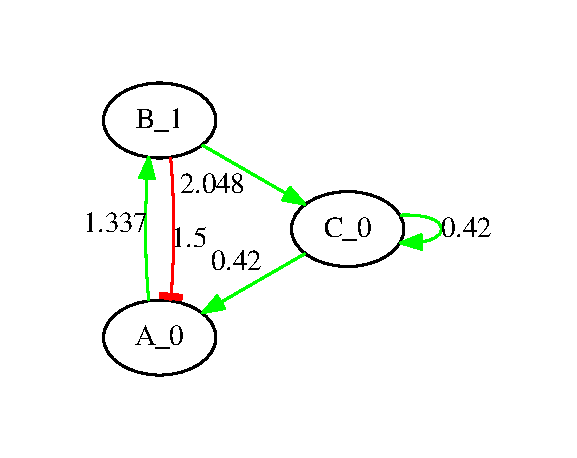
\includegraphics{example_weighted_graph}
        \caption{
            \label{ex_weighted_graph}
            Exemple d'un graphe orienté représentant la dynamique d'un réseau
            booléen à 3 noeuds. Les flèches vertes représentent des forces à
            coefficients positifs tandis que les flèches rouges ont des coefficients négatifs.
            Les nombres inscrits à côté des étiquettes des noeuds (séparé par
            un blanc souligné) représente le seuil que la somme des forces
            doit atteindre pour basculer d'un état à un autre.  Cela correspond
            à l'opposé de la force globale $-c_i$ dans la définition
            précédente.
        }
    \end{center}
\end{figure}

Si on considère que les mots $U_N$ identifiants les noeuds sont une suite de
nombres croissants, alors, comme il y a $N$ éléments et qu'on commence à
énumérer à partir du rang $0$, on peut conclure $ \forall i \in U_N, 0
\le i < N $ et surtout $ U_N = [\![0, N - 1]\!] $.  Dans la formule le mise à
jour \ref{func_maj_weight}, les coefficients $a_{i, j}$ peuvent alors être
regroupé dans une matrice $N\times N$.  Dans l'implémentation du programme, la
matrice a une taille réelle de $(N + 1)\times N$ car elle place sur la première
colonne le coefficient de force générale $c_i$.

\subsubsection{Ajout de délais dans le modèle}
Les réseaux de ce type avancent pas à pas et on considère dans cette
sous-partie que tous les noeuds des réseaux sont mis à jour à chaque fois pour
justifier la nécessité d'intégrer des délais. Si on prend comme exemple une
horloge composée de deux noeuds différents $CLK$ et $\overline{CLK}$.
L'utilisation de deux noeuds est obligatoire car dans la formule courante, il
n'y a des interactions seulement si les noeuds sont actifs. Donc ce n'est pas
possible d'avoir qu'un seul noeud qui oscille tout seul. Une fois qu'il s'est
désactivé, il ne peut plus se r\'eactiver. Cette horloge correspond à celle
présentée dans l'introduction \ref{intro_clock}. Un seul noeud peut être
actif à la fois. Les règles de mise à jour indiquent que $CLK$ active $\overline{CLK}$ et
se désactive tandis que $\overline{CLK}$ fait l'inverse. Cela fait bien
osciller l'horloge. Le problème, c'est que à chaque mise à jour, elle change d'\'etat.
Il n'est donc pas possible de créer une horloge oscillant avec une autre
fréquence.

Un moyen de permettre cela est de rajouter des noeuds de transition entre les
deux principaux comme une chaîne. Ainsi, lorsque $CLK$ veut activer
$\overline{CLK}$, il active à la place un noeud transitoire qui va ensuite, au
prochain pas, activer un autre noeud transitoire. Cela jusqu'à ce que
l'information arrive jusqu'à $\overline{CLK}$. Il doit aussi également y avoir
une transition au niveau de l'auto désactivation du noeud. Donc le dernier
noeud transitoire active $\overline{CLK}$ et désactive $CLK$. Une transition
différente peut également être placée sur le lien de $\overline{CLK}$ à $CLK$.
Elle peut avoir une longueur différente permettant ainsi de réguler le rapport
cyclique de l'horloge. Cette solution pose un problème dans le sens où elle
rajoute un nombre non-négligeable de noeuds. En effet, si le rapport cyclique
est proche de $0$ ou proche de $1$, alors il est obligatoire d'ajouter beaucoup
de noeuds. Or la taille de l'espace d'état d'un réseau booléen de taille $N$
est $2^N$. Il suffit donc dans cette horloge d'avoir une transition formée de
8 noeuds pour passer de $2^2=4$ états possibles à $2^{(2+8)}=1024$ états. Cette
solution est donc à proscrire généralement. Elle a toutefois l'avantage de
garder un résultat déterministe avec un réseau purement booléen.

Un autre moyen de rajouter un délai est de placer une loi de probabilité entre
les interactions qui choisirait entre l'activation et la désactivation de
celles-ci. Pour un délai de $d$ pas, alors la loi de probabilité devrait
n'activer l'interaction que une fois tout les $d$ temps en moyenne. La loi de
Bernouilli de paramètre $p = \frac{1}{d}$ vérifie cette hypothèse. Ainsi, dans
la formule \ref{func_maj_weight}, le terme $E_j(t)$ contrôlant l'activation de
l'interaction doit également gérer ce paramètre stochastique et devient
$E_j(t)\cdot 1\!\!1_{\mathbb{P}(X = 1)}$. Une interaction entre deux noeuds
n'est donc plus représentée par un simple coefficient scalaire mais par un
couple avec le coefficient et le paramètre de la loi de Bernouilli. Cette
solution est facile à mettre en place et ne prend pas beaucoup plus de mémoire
car il suffit d'avoir une matrice de couple. Mais elle a le désavantage d'être
stochastique et donc pas déterministe.

Il existe un dernier moyen qui a été ajouté au modèle qui est d'intégrer
directement un compteur à l'intérieur de chaque interaction. Ce compteur
s'incrémenterait à chaque pas durant lesquels le noeud originaire de la force
est actif. Une fois que ce compteur dépasse un seuil choisi correspondant au
délai souhaité, alors l'information de l'interaction est transmise. Le compteur
possède différentes propriétés qui peuvent être configurées dans l'interface de
la bibliothèque crée \footnote{Voir la classe \texttt{timed\_coef} dans le
fichier \texttt{bool\_network/dynamic/timed\_matrix\_model.h}}.  Un paramètre
permet de déterminer si oui ou non, le compteur doit être remis à $0$ une fois
que le seuil est dépassé. En effet, il peut y avoir différents types
d'interactions qui nécessitent pour certaine une réinitialisation du délai et
d'autre pour laquelle le délai ne représente qu'une période d'attente dans la
phase d'initialisation d'un processus. Seul le premier type est utilisé dans
les modèles pr\'esent\'es ici. Une autre caractéristique possible envisagée mais qui n'a
pas été gardé dans l'implémentation fournie est la mise en mémoire du compteur.
Pour l'instant, le compteur n'est incrémenté que lorsque le noeud est actif et
s'il ne l'est plus, le compteur est automatiquement remis à zéro. Il est
toutefois envisageable de garder l'état du compteur en mémoire même si le noeud
est désactivé. Cette solution n'a pas été gardé car elle n'est pas utilisée et
que la sémantique de délai simple ne colle pas vraiment à cette définition.
Cependant, le code est pensé pour qu'il soit possible de modifier facilement et
rapidement les types des coefficients stockés dans la matrice. Ainsi il est
théoriquement envisageable d'inclure des structures de données complexes dans
celle-ci tant que la structure suit des hypothèses défini dans la documentation
fournie. C'est possible grâce au développement de la bibliothèque en utilisant
des arguments de type template dans les patrons de conception.  Il est alors a
noter que l'état du réseau défini précédemment est pas tout à fait correcte
avec des délais de ce type. En effet, ce dernier ne comporte pas les compteurs
internes de la matrice qui n'est alors plus totalement statique. Si le réseau
doit être copié, il ne faut alors pas oublier ce détail à moins que seule la
dynamique soit a copier. Cela est géré automatiquement dans le code grâce à
l'opérateur de copie implicite du C++ qui se charge de faire une copie en
profondeur par valeur des données internes à l'objet. Cependant, si un des
constructeurs de copie ou même l'opérateur d'affectation est redéfini, la copie
en profondeur reviens à la charge de l'utilisateur.

\subsubsection{Choix des noeuds mis à jour}
Avec une modélisation de l'état du réseau et des règles de mise à jour, le
réseau n'est pas complètement défini. Il reste à définir comment et dans quel
ordre les règles sont appelées et combien le sont en même temps. En effet
certaines modélisations de machine ne peuvent pas être définies lorsque ce
choix n'est pas correctement configuré. La figure \ref{ex_diff_sync} montre
bien que cela change le graphe d'état et donc la dynamique obtenue par le
réseau. Dans le cas à gauche de la figure, deux modifications peuvent être fait
dans le même pas.  Lorsque l'un noeud est activé et l'autre désactivé (soit
l'état $01$ soit $10$), alors le réseau peut passer à l'autre directement. Les
états dans lesquels les deux noeuds sont tout les deux dans le même état ($00$
et $11$) sont des valeurs non-valides normalement. Mais ils sont affichés dans
le graphe d'état pour montrer toutes les possibilités. Dans le cas de la figure
de droite, un seul noeud peut être modifié. L'état $01$, pour passer à $10$
doit alors d'abord passer soit par $00$ ou $11$. Or à partir de ces états, la
dynamique n'est pas définie (ici elle ne fait que boucler l'état sur lui-même).
Même en considérant que c'est possible de conclure de la prochaine valeur pour
passer à $10$ comme convenu (cela casserait le fait que le système est
Markovien puisqu'il faudrait se souvenir de la trace parcourue), il y aurait un
moment pendant lequel l'horloge aurait un état invalide.

\begin{figure}[position]
    \begin{center}
        \begin{minipage}[c]{.49\linewidth}
            \centering
            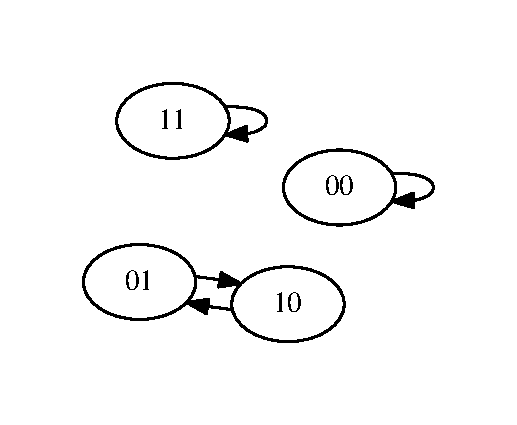
\includegraphics[scale=0.85]{bool_net_async}
        \end{minipage}
        \hfill
        \begin{minipage}[c]{.49\linewidth}
            \centering
            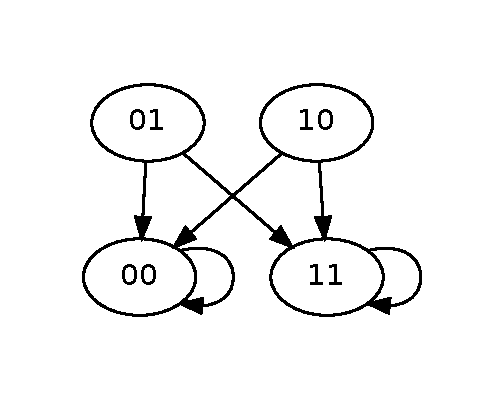
\includegraphics[scale=0.85]{bool_net_sync}
        \end{minipage}
        \caption{
            \label{ex_diff_sync}
            Graphe d'état d'une horloge avec, à gauche, deux modifications
            possibles par pas et, à droite, une seule modification possible.
        }
    \end{center}
\end{figure}

Il est également à noter que dans le cas où un seul des noeuds est modifié,
dans le graphe d'état, il existe des états qui ont deux successeurs. Cela
montre alors que ce type de graphe d'état n'est pas déterminé pour l'instant et
qu'il faut définir une loi de choix du chemin pour rendre le graphe déterminé
totalement. C'est également cette loi qui sert à combler le manque dans la
modélisation du réseau. Dans le cas où le nombre de modification possible faite
par pas est égale à la taille du réseau, alors le graphe est déjà entièrement
déterminé.

La solution utilisée est, à partir d'un état du réseau, de simuler un pas et de
lister toutes les modifications possibles sans ex\'ecuter les mises à jour. Une loi uniforme choisi alors un
certain nombre prédéfini de modifications qui seront effectives. Ce nombre est
totalement paramétrable et se configure pour adopter la dynamique et
l'évolution voulue dans le système. Lorsque ce nombre est égal à la taille du
réseau, alors le résultat est déterministe. Dans le cas inverse, l'avancée dans
le graphe d'état est aléatoire et il est possible, à partir d'un même état
initial d'arriver à des points de convergence dans le graphe totalement
différents et de parcourir des chemins opposés. L'algorithme pour la fonction
de choix des modifications est donc le suivant pour un choix de $K$
modifications :

\begin{multline}
    \mbox{Soit } L \mbox{ un sous-ensemble aléatoire des indices des
    modifications : } \\
    L \subset \left\{i, \forall i \in U_N | E_i(t + 1) \ne E(t)\right\} \\
    \Omega(L) \le K \\
    \forall i \in U_N, E'_i(t + 1) = \left\{\begin{array}{rl}
        E(t + 1), & \mbox{si } i \in L \\
        E(t), & \mbox{sinon}
    \end{array}\right.
\end{multline}

L'état après transformation complète est l'ensemble des $E'_i$. \\

Une trace du chemin parcouru dans le graphe d'état est gardé en mémoire au
niveau de l'implémentation. Cette trace sert d'historique et permet de calculer
instantanément l'état après un certain nombre de pas lorsque la machine est en
train de boucler. En effet, si un nouvel état fait partie de l'historique des
états visités, cela signifie qu'il y a une boucle dans le graphe d'état. On
peut alors, grâce à l'historique, sauter directement au prochain état voulu
même si on demande une avancée d'un nombre de pas très grand. Il n'y a pas
besoin de recalculer tous les états intermédiaires. Cependant, comme dit plus
haut, en partant d'un état, il est possible de passer par un chemin différent.
Cela empêche l'utilisation directe de l'historique. Pour mélanger l'aléatoire
de l'avancée et le déterminisme de l'historique, il est possible de dire qu'on
ne veut considérer être dans une boucle du graphe uniquement après un certain
nombre de pas à être dans la même boucle. Plus ce nombre est élevé et plus on
est sûr qu'il n'y a aucun moyen de sortir de la boucle. On peut alors
considérer à utiliser l'historique. Encore une fois ce nombre est paramétrable
et est laissé au choix de l'utilisateur. De plus, dans les modèles utilisés, la
plupart des boucles sont des singletons. Cela permet de conclure facilement sur
le bouclage. Aussi, le temps d'attente est aussi utile lors de l'utilisation de
modèle possédant des délais. En effet, les formules utilisées ne prennent en
compte que l'état et le compteur temporel ne fait pas partie de l'état du
réseau comme il est défini. Il faut donc au moins attendre le délai maximum
avant de conclure sur la convergence des états dans une boucle.

\subsection{La machine de destin cellulaire}
\subsubsection{Présentation}
Cette machine permet sa savoir si la cellule survie ou meurt en fonction de la
présences des cytokines \texttt{TNF} et \texttt{FAS}. Le réseau utilisé est
inspiré de la simplification du modèle de Calzone et collègues \cite{calzone2010}. Ce
modèle utilise des fonctions de mise à jour booléennes. Il a donc fallu
transformer ces règles en une matrice de coefficients \footnote{Cette matrice
est disponible dans la source du programme dans le fichier
\texttt{bool\_network/models/fadd.cpp}}. Il n'y a aucun délai dans ce modèle
donc les coefficients de la matrice ne sont que des scalaires. 

\begin{figure}[position]
    \begin{center}
        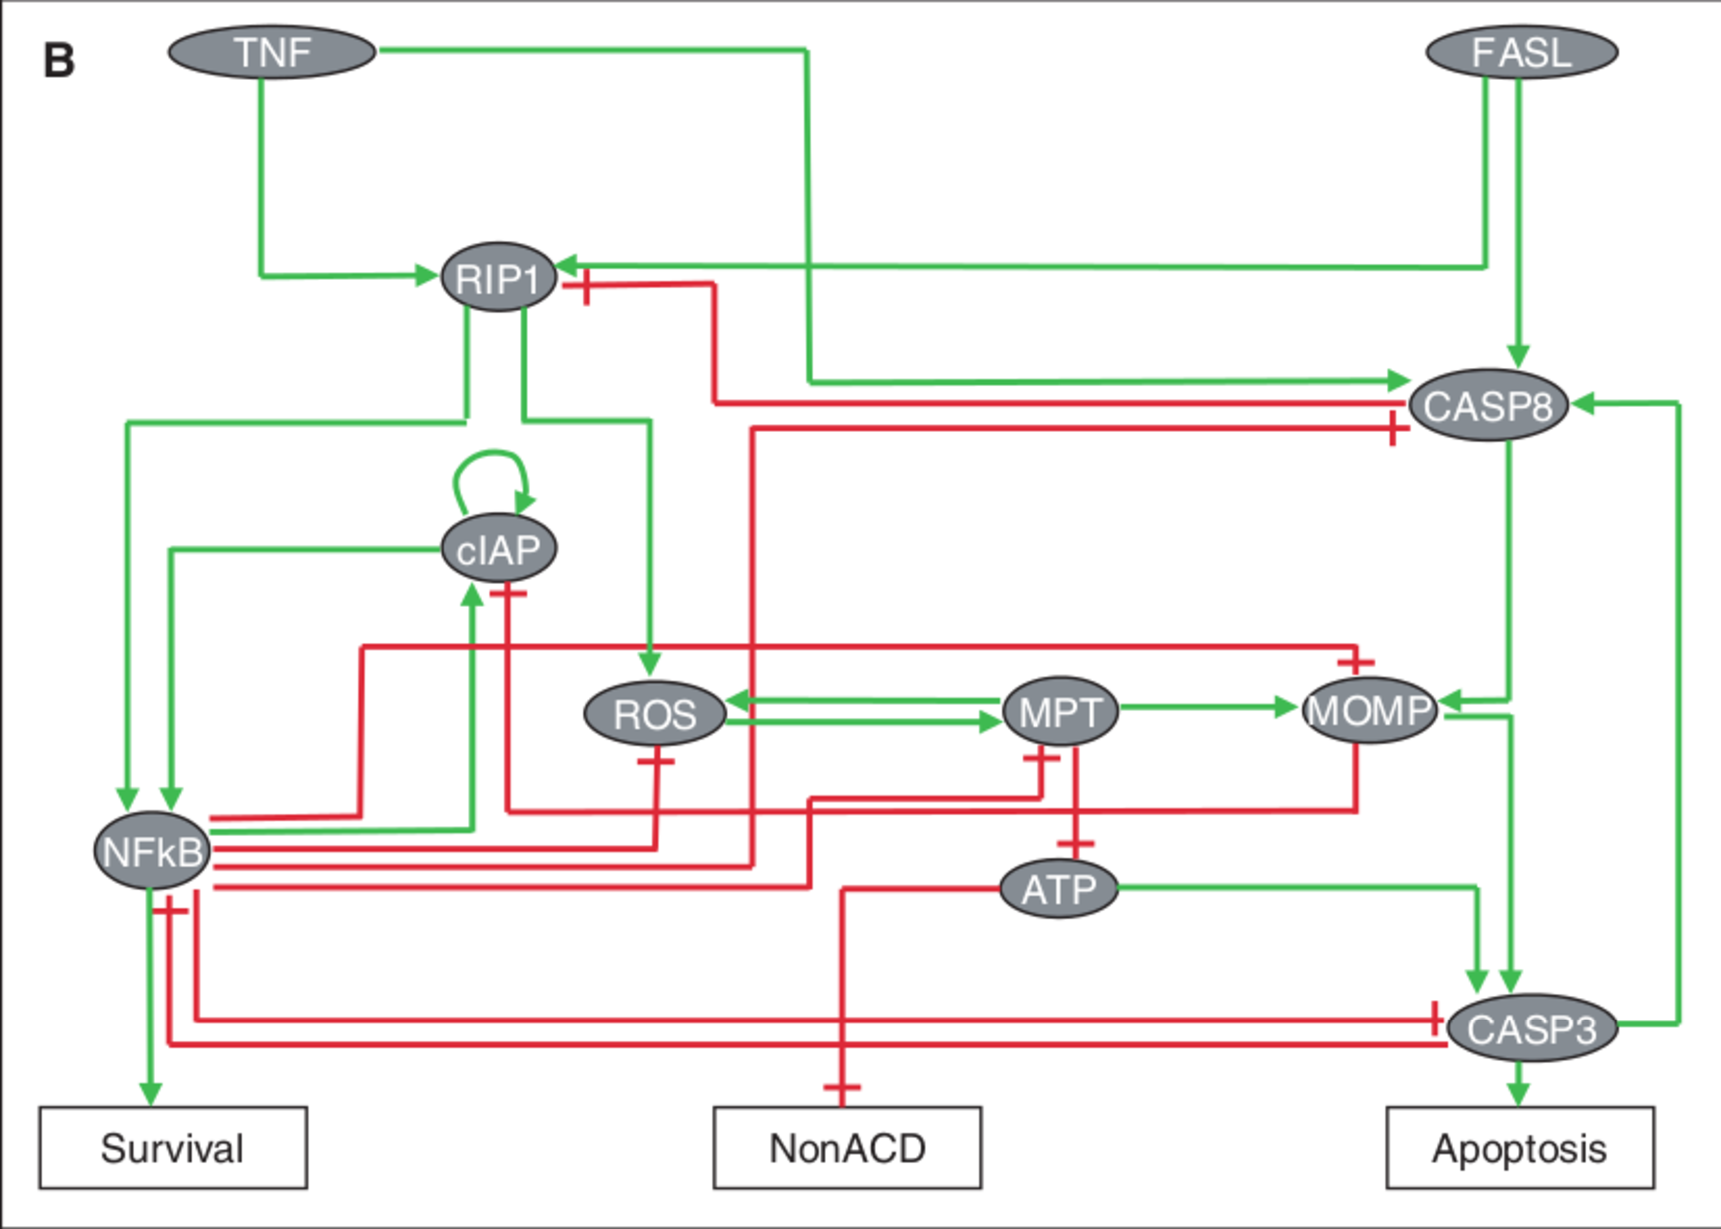
\includegraphics[scale=0.4]{net_fadd}
        \caption{
            \label{net_fadd}
            Réseau booléen de la machine contrôlant le destin cellulaire.
            Figure reproduite de la source \cite{calzone2010}
        }
    \end{center}
\end{figure}

La figure \ref{net_fadd} montre les interactions entre les noeuds du réseau.
Les deux entrées sont au-dessus et les trois sorties en bas. Ce schéma montre
les différentes conditions de choix du destin. La survie survient lorsqu'il y a
du $NF\kappa B$ tandis que l'absence d'\texttt{ATP} ou la présence de
\texttt{CASP3} entraîne la mort. Un seul choix peut être fait entre la vie et
la mort. Dans le cas où plus d'une des conditions est remplies, on dit que la
cellule est sur un résultat trivial qui ne nous intéresse pas. On ne peut pas
conclure du destin.

\subsubsection{Simulation du modèle}
Pour simuler le réseau, l'état initial est prédéfini. Tous les noeuds sont
désactivés sauf l'\texttt{ATP} et le \texttt{MTP}. En effet, si on considère
une cellule vivante comme point de départ, cela signifie qu'elle a de l'énergie
et donc de l'\texttt{ATP}. Les entrées \texttt{TNF} et \texttt{FAS} sont
ensuite modifiée puis la simulation est faite. Comme l'état initial est défini,
pour éviter de n'avoir que 4 solutions possibles (les 4 possibilités de choix
des entrées), l'avancement est aléatoire. La fonction de choix du réseau
n'effectue que une seule modification par pas. Ainsi, des chemins différents
peuvent être parcourus et différents points de convergences sont atteints.

\subsubsection{Définition des mutations possibles}
Le modèle utilisé propose l'implémentation et le changement des règles de façon
à reproduire des mutations possibles biologiquement. Celles-ci changent alors
la dynamique du réseau et permet d'obtenir des résultats sensiblement
différents.  Par exemple, certaines mutations peuvent activer la surexpression
des protéines de la famille des caspases. Ce type de mutation va alors
entraîner un nombre beaucoup plus important de mort par apoptose. D'autres
peuvent également limiter la mort de la cellule rallongeant largement la durée
de vie de la population.  Une cellule peut être mutée lors de sa création
(initialement ou par mitose) avec une certaine probabilité. Il serait aussi
possible de créer une autre machine booléenne exclusivement dédiée au choix de
la mutation à prendre. Le choix de la mutation et l'intégration dans la cellule
n'a pas pu être inclut dans le travail fourni par manque de temps. Cependant
les modèles des machines de choix du destin mutées sont présents dans le
programme. Ils peuvent d'ailleurs être utilisés tout de même si on considère
que toute la population à la même mutation.

La liste des mutations ainsi que leur effets est montrée dans la partie
résultat \ref{section_resultat}.

\subsection{Détermination de la phase dans le cycle cellulaire}

\begin{figure}[position]
    \begin{center}
        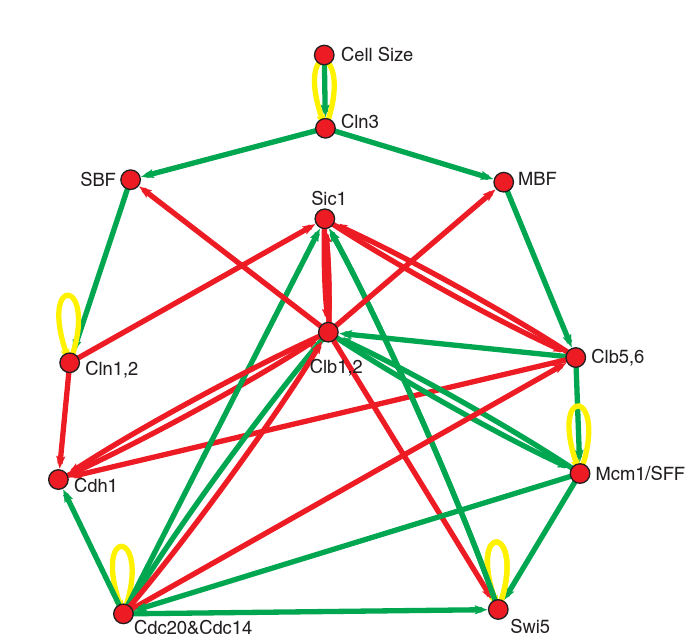
\includegraphics[scale=0.335]{net_cycle}
        \caption{
            \label{net_cycle}
            Réseau booléen de la machine du cycle cellulaire. Les flèches
            vertes et rouges indiquent les interactions positives et négatives
            entre les noeuds. Les flèches jaunes correspondent à une auto
            dégradation du noeud.
            Figure reproduite de la source \cite{li2004}
        }
    \end{center}
\end{figure}

La machine  pour déterminer la phase dans le cycle cellulaire reprend la source
\cite{li2004}. Ce modèle correspond à un réseau booléen du cycle de vie d'une
levure. Ce modèle n'a qu'une entrée qui est le dépassement d'une taille seuil
par la cellule. On peut voir sur la figure \ref{net_cycle} que ce noeud nommé
\texttt{Cell Size} est placé en haut et active en cascade ses voisins. Aussi,
le paramètre $K$ de la fonction de choix est égale au nombre de noeuds $N$ dans
le réseau. Donc toutes les modifications possibles sont effectuées à chaque
itération de la simulation. Ce modèle est donc déterministe ce qui permet, par
sa taille réduite ($N = 12$), de connaître tous les résultats possibles et de
vérifier ainsi des propriétés sur le réseau.

Il existe dans ce système une notion d'auto-dégradation de certains noeuds. Les
noeuds soumis à ce genre de phénomènes sont ceux qui ne possède pas
d'interactions négatives. Ils sont alors constamment maintenus une fois
activés. Cette dégradation désactive le noeud après un certain moment sans
activations de celui-ci par les autres (ou de lui-même s'il participe à sa
propre activation). Cela se justifie car l'information stockée dans le réseau
est booléen et il n'est alors pas possible de connaître la quantité ou la
concentration des protéines. Or sans production d'une protéine, celle-ci est
d\'egradée et disparait. Cela se traduit dans le réseau booléen par une
interaction négative du noeud en question sur lui-même. Le coefficient est
petit car la priorité de la dégradation est faible par rapport à
l'activation. De plus, celle-ci peut être sur plusieurs itérations du réseau.
L'utilisation des délais est alors possible pour permettre de réguler la
``perte'' de protéines.

Les coefficients positifs de la matrice sont les mêmes et sont notés $A_g$.
C'est la même chose pour les coefficients négatifs qui sont alors notés $A_r$.
Aussi, tous les délais de dégradations sont les mêmes  pour les noeuds en
questions et ont pour valeur $T_d$. Ces trois valeurs sont modifiables dans le code grâce
à des paramètres à la construction \footnote{voir la classe
    \texttt{bn::models::yeast} dans le fichier
\texttt{include/bool\_network/models/yeast.h}}.

Une propriété est remarquée tant que $A_g \ge A_r$ et $T_d > 0$. En effet, il
existe 7 états dans le graphe d'état du réseau vers lesquels tous les autres
états convergent. Ils sont les même quelques soit les valeurs des trois
paramètres tant qu'ils suivent la condition. Ces bassins d'attractions sont
donc utile pour prévoir le comportement de la dynamique du système et savoir à
quel résultat s'attendre. Des tests unitaires peuvent ainsi être écrit pour
vérifier cela. De plus, l'un de ces bassins de convergence est majoritaire par
rapport au autres. Travailler dans ce seul bassin permet alors d'avoir la même
convergence. De plus, lorsque le système a convergé vers cet état, l'activation
du noeud d'entrée \texttt{Cell Size} rend le réseau booléen toujours stable sur
ce bassin. Cet état peut alors servir d'état initial et la convergence comme
état final. L'activation de l'entrée permet alors de réamorcer la simulation du
cycle cellulaire.

\subsection{Création d'un modèle bistable}
La machine dédiée au choix entre la différentiation ou le renouvellement de la
cellule est un système bistable. Ce choix est alors traité au niveau de
l'interface avec la cellule en complément à la machine représentant le cycle
cellulaire. Cette dernière décrit le moment où la cellule est mitotique et
cette machine dicte le choix à faire sur lors de la division. Cet aspect n'est,
toutefois, pas géré par le code pour le moment car le choix du type de mutation
n'a pas pu être fait. Lorsqu'il y a mitose d'une cellule, celle-ci se
renouvelle à l'identique pour le moment.

Les deux états bistables représentent la présence ou l'absence de la protéine
\texttt{GATA-1} dans la cellule. Cela est géré par un réseau booléen composé de
deux noeuds. L'un représentant le \texttt{GATA-1} et l'autre l'\texttt{EPO}. Le
seul contrôle se fait sur le noeud de l'\texttt{EPO}. Lorsque celui-ci est
activé, il active \texttt{GATA-1} après un certain délai paramétrable. Ainsi,
même lorsqu'il n'y a plus la détection de la présence d'\texttt{EPO},
l'information est tout de même transmis et gardé en mémoire. Cette mémoire peut
alors ensuite être réinitialisée pour établir un nouveau choix pour le nouveau
cycle cellulaire. % TODO faire la machine EPO

Par définition, le choix apporté par ce modèle doit être plus rapide que la dur\'ee
du cycle cellulaire. Cela est totalement réglable dans l'interface faite entre
la bibliothèque de machine booléenne fournie et la définition finale du modèle
de la machine. De plus, pour permettre au noeud du \texttt{GATA-1} de s'activer
dès que l'attente soit remplie, les deux modifications des deux noeuds doivent
être effectives. Ce système est donc complètement déterministe.

\subsection{Élaboration d'une horloge circadienne}
La machine servant d'horloge est une simple horloge booléenne à deux états.
Cela signifie que ce n'est qu'un signal périodique avec un état haut pendant un
certain temps $T_{on}$ puis un autre état bas pendant une durée $T_{off}$.
Ces deux paramètres sont réglables dans l'implémentation faite \footnote{Voir
    la structure de donnée \texttt{bn::models::clock\_info} dans le fichier
\texttt{include/bool\_network/models/clock.h}}. Il existe également un autre
paramètre permettant de modifier le déphasage du signal d'un certain temps.

Le réseau booléen utilisé est celui montré sur la figure \ref{net_clock}.
Celui-ci est composé de deux noeuds. Il est obligatoire d'avoir deux noeuds
pour faire osciller l'horloge car il ne peut y avoir des changements et des
modifications dans un réseau booléen seulement si au moins un noeud est activé.
L'évolution de l'oscillateur est alors simulée en utilisant un couple de noeud
qui clignotent. Pendant que l'un des noeuds est activé, l'autre est désactivé.
Si les deux sont dans le même état, c'est qu'il y a une erreur dans la
simulation. Lorsqu'un noeud est activé, il va activer l'autre et se désactiver
en même temps. En général, pour pouvoir modifier le rapport cyclique de
l'horloge, un modèle de réseau booléen disposant de délais est utilisé. Les
délais pour l'activation de l'autre noeud et l'auto-désactivation est alors le
même pour synchroniser le passage à l'état haut et celui à l'état bas.

\begin{figure}[position]
    \begin{center}
        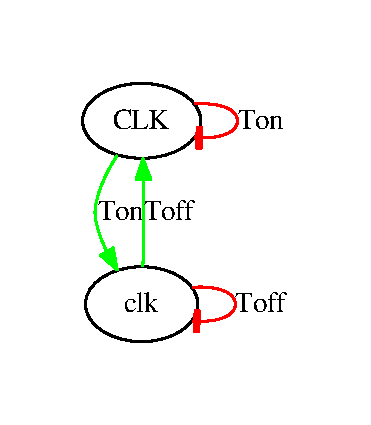
\includegraphics[scale=1.0]{bool_net_clock}
        \caption{
            \label{net_clock}
            Schéma du réseau booléen de l'horloge binaire servant de base pour
            l'horloge circadienne de la cellule.
        }
    \end{center}
\end{figure}

Dans l'implémentation, une sécurité est installée pour empêcher l'utilisateur
de pouvoir dérégler cette synchronisation. En effet, il est possible de forcer
l'activation d'un des noeuds. La s\'ecurit\'e désactivera alors automatiquement
l'autre noeud. L'activation forcée permet par exemple la simulation de l'excitation de la
cellule par une source extérieur comme la présence de la lumière.

\subsection{Mise en place des machines dans la cellule puis dans la population}
Le code est conçu pour que les machines soient de le plus générales
possible\footnote{Voir la documentation de la bibliothèque template fournie en
annexe.}. Cela utilise des concepts avancés de la programmation template en
C++ ainsi que du paradigme de programmation orientée objet. En effet, toute la
dynamique et les modèles de bases sont encapsulés dans une bibliothèque
crée et fournie avec ce rapport. Une surcouche est alors faite en parallèle de la classe de la
cellule booléenne afin de spécifier totalement les données manquantes et de
paramétrer correctement les modèles de bases pour reproduire fidèlement la
dynamique du système voulu.

Chacune des interfaces est alors utilisée dans l'implémentation de la cellule
booléenne et intégrée à l'intérieur de celle-ci. Les entrées et les sorties des
réseaux booléens sont alors connectées aux éléments correspondants dans la
cellule. Également, pour simuler l'intégration de la cellule au sein de la
population, des signaux représentés par des nombres sont transmis entre chaque
cellule en contact avec d'autres.

Les signaux transmis représentent biologiquement des cytokines. La transmission
des données entre les cellules n'est pas a priori gérée dans le modèle de
cellule booléenne car le signal booléen est transmis par moyenne et est donc
représenté comme un signal réel plutôt que bool\'een à l'extérieur de la cellule.

Les états intracellulaires des cellules sont mis à jour par le module de
simulation à intervalles de temps constants $\Delta t$. Ceci permet de gérer
les interactions entres cellules et les mouvements cellulaire. Ces interactions
ne sont pas l'objet de ce travail et les détails d'implémentation sont omis
ici. Par contre, le fait d'avoir un pas de temps $\Delta t$ à l'échelle de la
population impose de fait une échelle de temps sur la dynamique des réseaux
booléens. Il est donc nécessaire de pouvoir remettre à l'échelle la progression
temporelle des machines. Au début de l'implémentation, l'avancé ne pouvait se
faire qu'avec des pas entiers pour suivre la définition des réseaux booléens.
Il n'était donc pas possible d'avancer moins d'une unité de temps. L'unité
utilisée ici est l'heure et le $\Delta t$ correspond à $0.2$h. Ces paramètres
n'étaient pas compatibles avec les réseaux intracellulaires. Une loi de Poisson
a donc été utilisé pour déterminer le nombre de mises à jour effectuées à
chaque pas de temps $\Delta t$. Le paramètre de la loi de Poisson $\mu = \Delta
t / \tau_M$, où $\tau_M$ est l'échelle de temps de la machine $M$ (c.-à-d. la
durée intrinsèque d'un pas de temps de la machine). Dernièrement, le module de
simulation est devenu une surcouche complète à l'implémentation des réseaux
booléens. Le temps interne de ce module est donc dissocié de celui du réseau.
Cela permet alors de faire des avancés avec des pas non-entiers. D'autre lois
peuvent être utilisées. Pour l'instant, chaque machine avance d'un pas $\Delta
t / \tau_M \pm \epsilon$ où $\epsilon$ est un écart aléatoire suivant une loi
uniforme réduit à un intervalle défini.

Un travail sur des essais de synchronisation des horloges
circadiennes a été mené. Pour rendre le signal moins artificiel, la p\'eriode de l'horloge 
a \'t\'e adapt\'ee et mise à l'\'echelle par la
loi de poisson, qui est utilisé pour d\'eterminer le nombre de pas à effectuer par
itération intracellulaire pour la machine d'horloge. Chaque horloge dans
chaque cellule n'avance donc pas au même rythme réellement. Une synchronisation
de ces horloges doit donc être faite pour limiter les écarts entre les
cellules.

Les flags interne de la cellule sont également modifiés par les états des
sorties des machines booléennes. Par exemple la machine du destin cellulaire
permet de garder à jour le flag indiquant si la cellule survie ou si elle va
mourir. Aussi, la fonction gérant la mitose de la cellule utilise également la
machine représentant le cycle cellulaire et la machine bistable choisissant
entre différentiation et renouvellement.

La machine de destin cellulaire est fonctionnelle et l'intégration et la
modification du flag dans la cellule sont gérées. Cependant, la mort de la cellule
n'est pas encore gérée totalement au sein de la population.

Il est possible de rajouter d'autres composants sous forme de machines
booléennes et de gérer la connexion avec l'environnement interne et externe à
la cellule. De plus, des connexions entre différents réseaux booléens est
également possible. L'implémentation du code est faite pour que la
réutilisation du code est sa prise en main soit la plus facile possible pour un
autre développeur. En effet, des exemples ont été ajouté dans la bibliothèque
pour montrer comment utiliser les modèles et les modules de dynamique et de
simulation existants. De plus, chaque module créé pour le moment a été testé
pour vérifier les propriétés de ceux-ci (voir les résultats
\ref{section_resultat}).

\newpage
\section{Résultat}
\label{section_resultat}
\subsection{Tests et essais sur l'implémentation d'un réseau booléen}
Beaucoup de tests unitaires et fonctionnels ont été fait sur l'élaboration de la
partie dynamique et et de la partie simulation de la bibliothèque gérant les
machines à états booléens avant de créer le moindre type de modèle quelconque.
Ces tests sont visibles dans le dossier \texttt{tests} du dossier de la
bibliothèque fournie.

Le premier regroupement de tests étudie les différents comportements des
réseaux booléens modélisés par une matrice de coefficients scalaires. Pour être
sûr que le résultat soit bien déterminé, les tests utilisent des réseaux
booléens complètement déterministes. Bien sûr des tests sur des modèles
stochastiques ont été fait en essayant de reproduire les résultats de la
littérature utilisée. Les premiers tests ne servent qu'à vérifier que la
définition de la dynamique soit juste grâce aux cas triviaux. En effet, le
réseau n'a qu'un seul noeud et vérifie l'interaction du noeud avec lui-même et
l'utilisation de la force globale sur celui-ci. Cela vérifie la stabilité du
système et de l'implémentation. Ensuite, des réseaux à 2 noeuds sont testés.
D'abord reproduisant les même cas qu'avec un seul noeud puis chacun agissant
sur l'autre. Enfin, les derniers tests vérifient la capacité du programme à
prévoir les comportements cycliques d'un réseau. D'abord dans le cas d'un
oscillateur à deux noeuds puis avec quatre noeuds différents. Les valeurs
attendues sont vérifiées jusqu'à un nombre d'itération $N = 1000$ \footnote{Tous
ces différents tests sont visibles dans le fichier
\texttt{tests/matrix\_model/main.cpp}. De nombreux commentaires expliquent la
réalisation et la justification de chaque test.}. Ce nombre est modifiable et
permet de tester avec un nombre d'itération plus grand. On considère que cela
suffit car le modèle est cyclique sur moins de 10 états normalement.
L'historique du réseau booléen est donc utilisé pour déterminer instantanément
les états après une vingtaine d'itération. C'est cet aspect qui est testé.

Le deuxième regroupement de tests \footnote{Voir
\texttt{tests/timed\_matrix\_model/main.cpp}} vérifie le comportement des
réseaux booléens utilisant des délais déterministes. Les mêmes vérifications
que pour le premier regroupement sont faits avec des délais de 0 pour vérifier
que le cas trivial est valide. Des tests vérifiant les délais sont ensuite
faits.  Les premiers sont également triviaux et ne sont que les précédents avec
un délai. Comme seule la convergence est vérifiée, le résultat obtenu doit
être le même qu'avant même avec un déphasage du temps pour obtenir le résultat.
Dans le cas des tests faisant intervenir des réseaux ayant une dynamique
cyclique, le déphasage doit être pris en compte. Les vérifications des états
convergents se fait donc au modulo près.

Il n'y a pas de tests unitaires vérifiant les caractéristiques de chacun des
modèles de base créés. Seulement des tests fonctionnels servant d'exemples
d'utilisation du code. Ces derniers sont présentés dans les sections suivantes.

\subsection{Simulation du destin d'une cellule}
Le réseau booléen servant à modéliser la réponse à l'activation des récepteurs
\texttt{TNF} et \texttt{FAS} à d'abord était modélisé en utilisant directement
les règles booléennes \footnote{Visible dans les traces du dépôt \texttt{SVN}}.
Après conversion en réseau booléen à matrice, les tests ont été refait et
réadapté \footnote{Voir les dossiers \texttt{examples/converge\_fadd/} et
\texttt{examples/decision\_fadd/}}. Les résultats obtenus étaient les mêmes
qu'avant montrant bien que les deux réseaux sont équivalant.

Ce modèle est stochastique. La vérification de l'exactitude des résultats s'est
donc fait en testant un nombre élevé de fois pour voir la moyenne de la
dynamique. Pour un test, l'état de départ est identique. Il y a en tout quatre
points de départ (car il y a deux entrées). Il y a donc quatre tests. On sait
que le système converge rapidement (il faut à peu près une vingtaine
d'itérations). Donc la simulation avance d'un nombre supérieur à cette
estimation. Dans ce cas, elle avance de 1000 pas. Après la simulation, nous
étudions la valeur des noeuds de sorties pour établir le choix entre la survie,
la mort par apoptose, celle par nécrose, et le cas indéterminé. Cette
simulation est refaite 10000 fois avec les mêmes conditions. On reporte alors
le pourcentage de chaque choix dans un graphique.

\begin{figure}[position]
    \begin{center}
        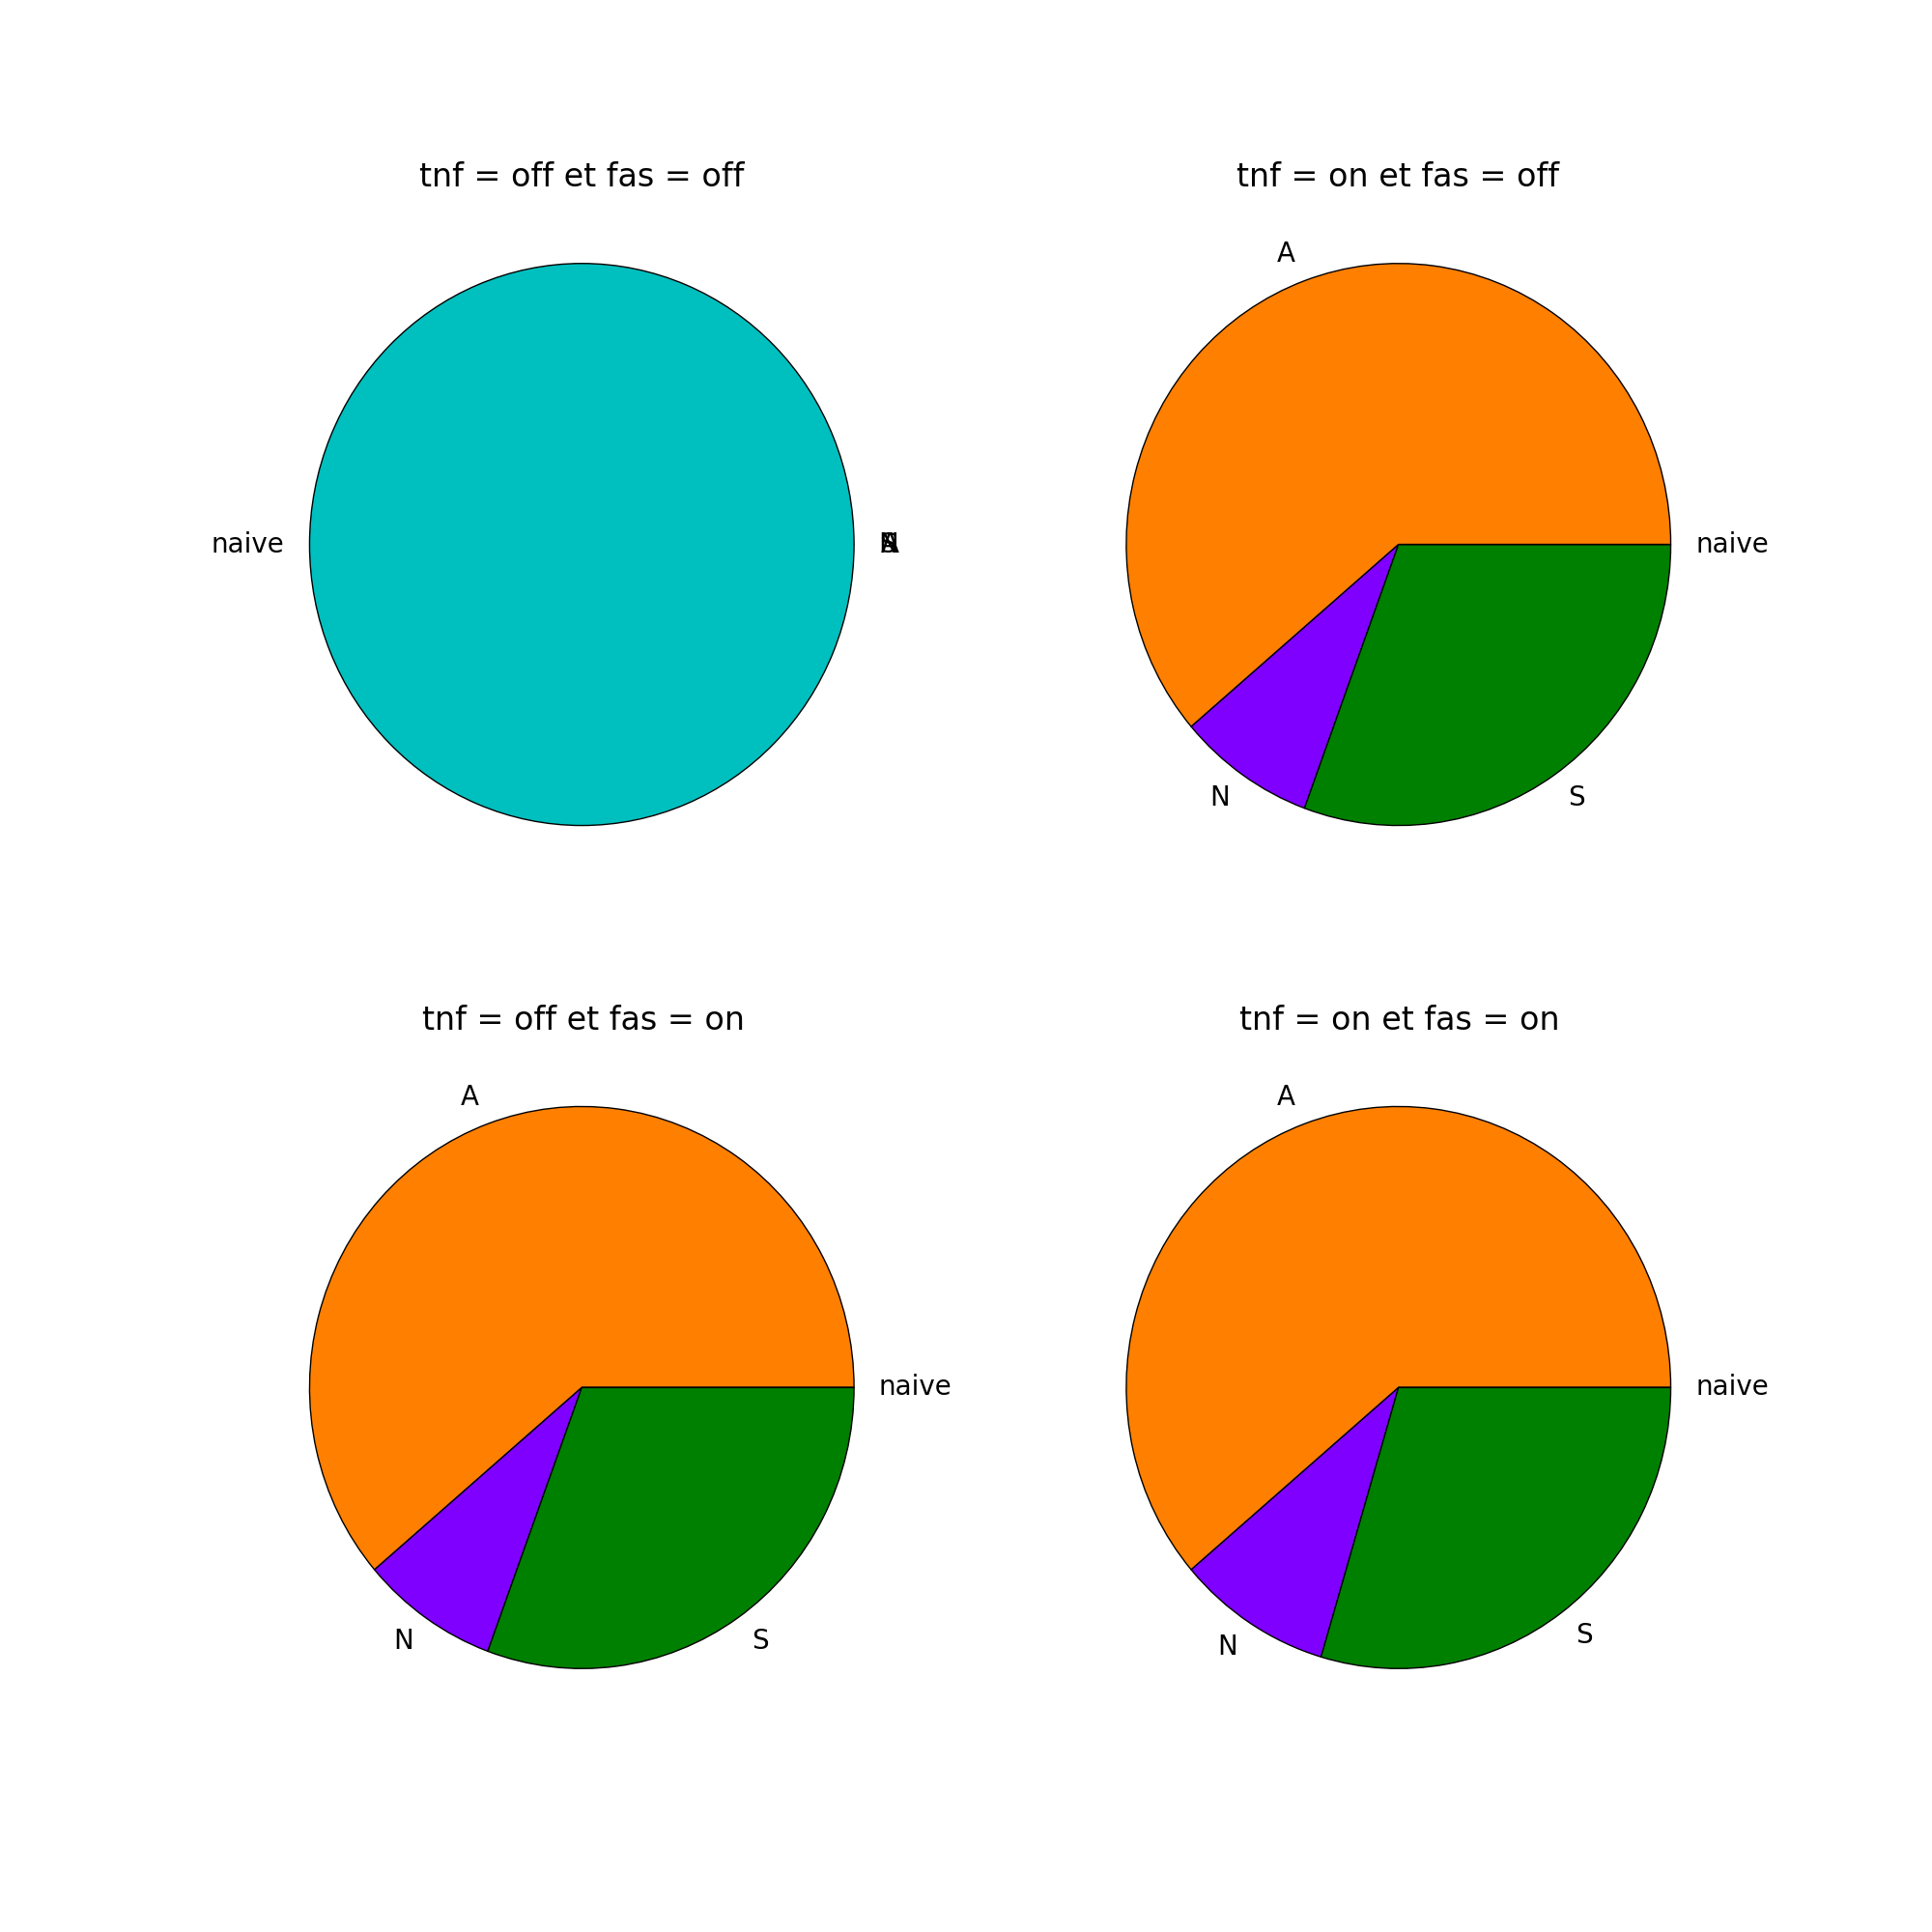
\includegraphics[scale=0.27]{result_fadd}
        \caption{
            \label{result_fadd}
            Résultats obtenus lors de la simulation du modèle de base du choix
            de destin cellulaire. En orange : mort par apoptose. En violet :
            mort par nécrose. En vert : survie. En cyan : choix indéterminé.
        }
    \end{center}
\end{figure}

La figure \ref{result_fadd} montre la modification des paramètres sur la
dynamique du modèle de base. Les figures (\ref{tnf0_fas0}, \ref{tnf1_fas0},
\ref{tnf0_fas1}, \ref{tnf1_fas1}) montrent également les résultats sur les
modèles de choix de destin pour les cellules mutantes. Le nom de chaque
mutation est indiqué au-dessus de sa figure. L'étiquette \texttt{wild\_type}
correspond au modèle de base.

\begin{figure}[position]
    \begin{center}
        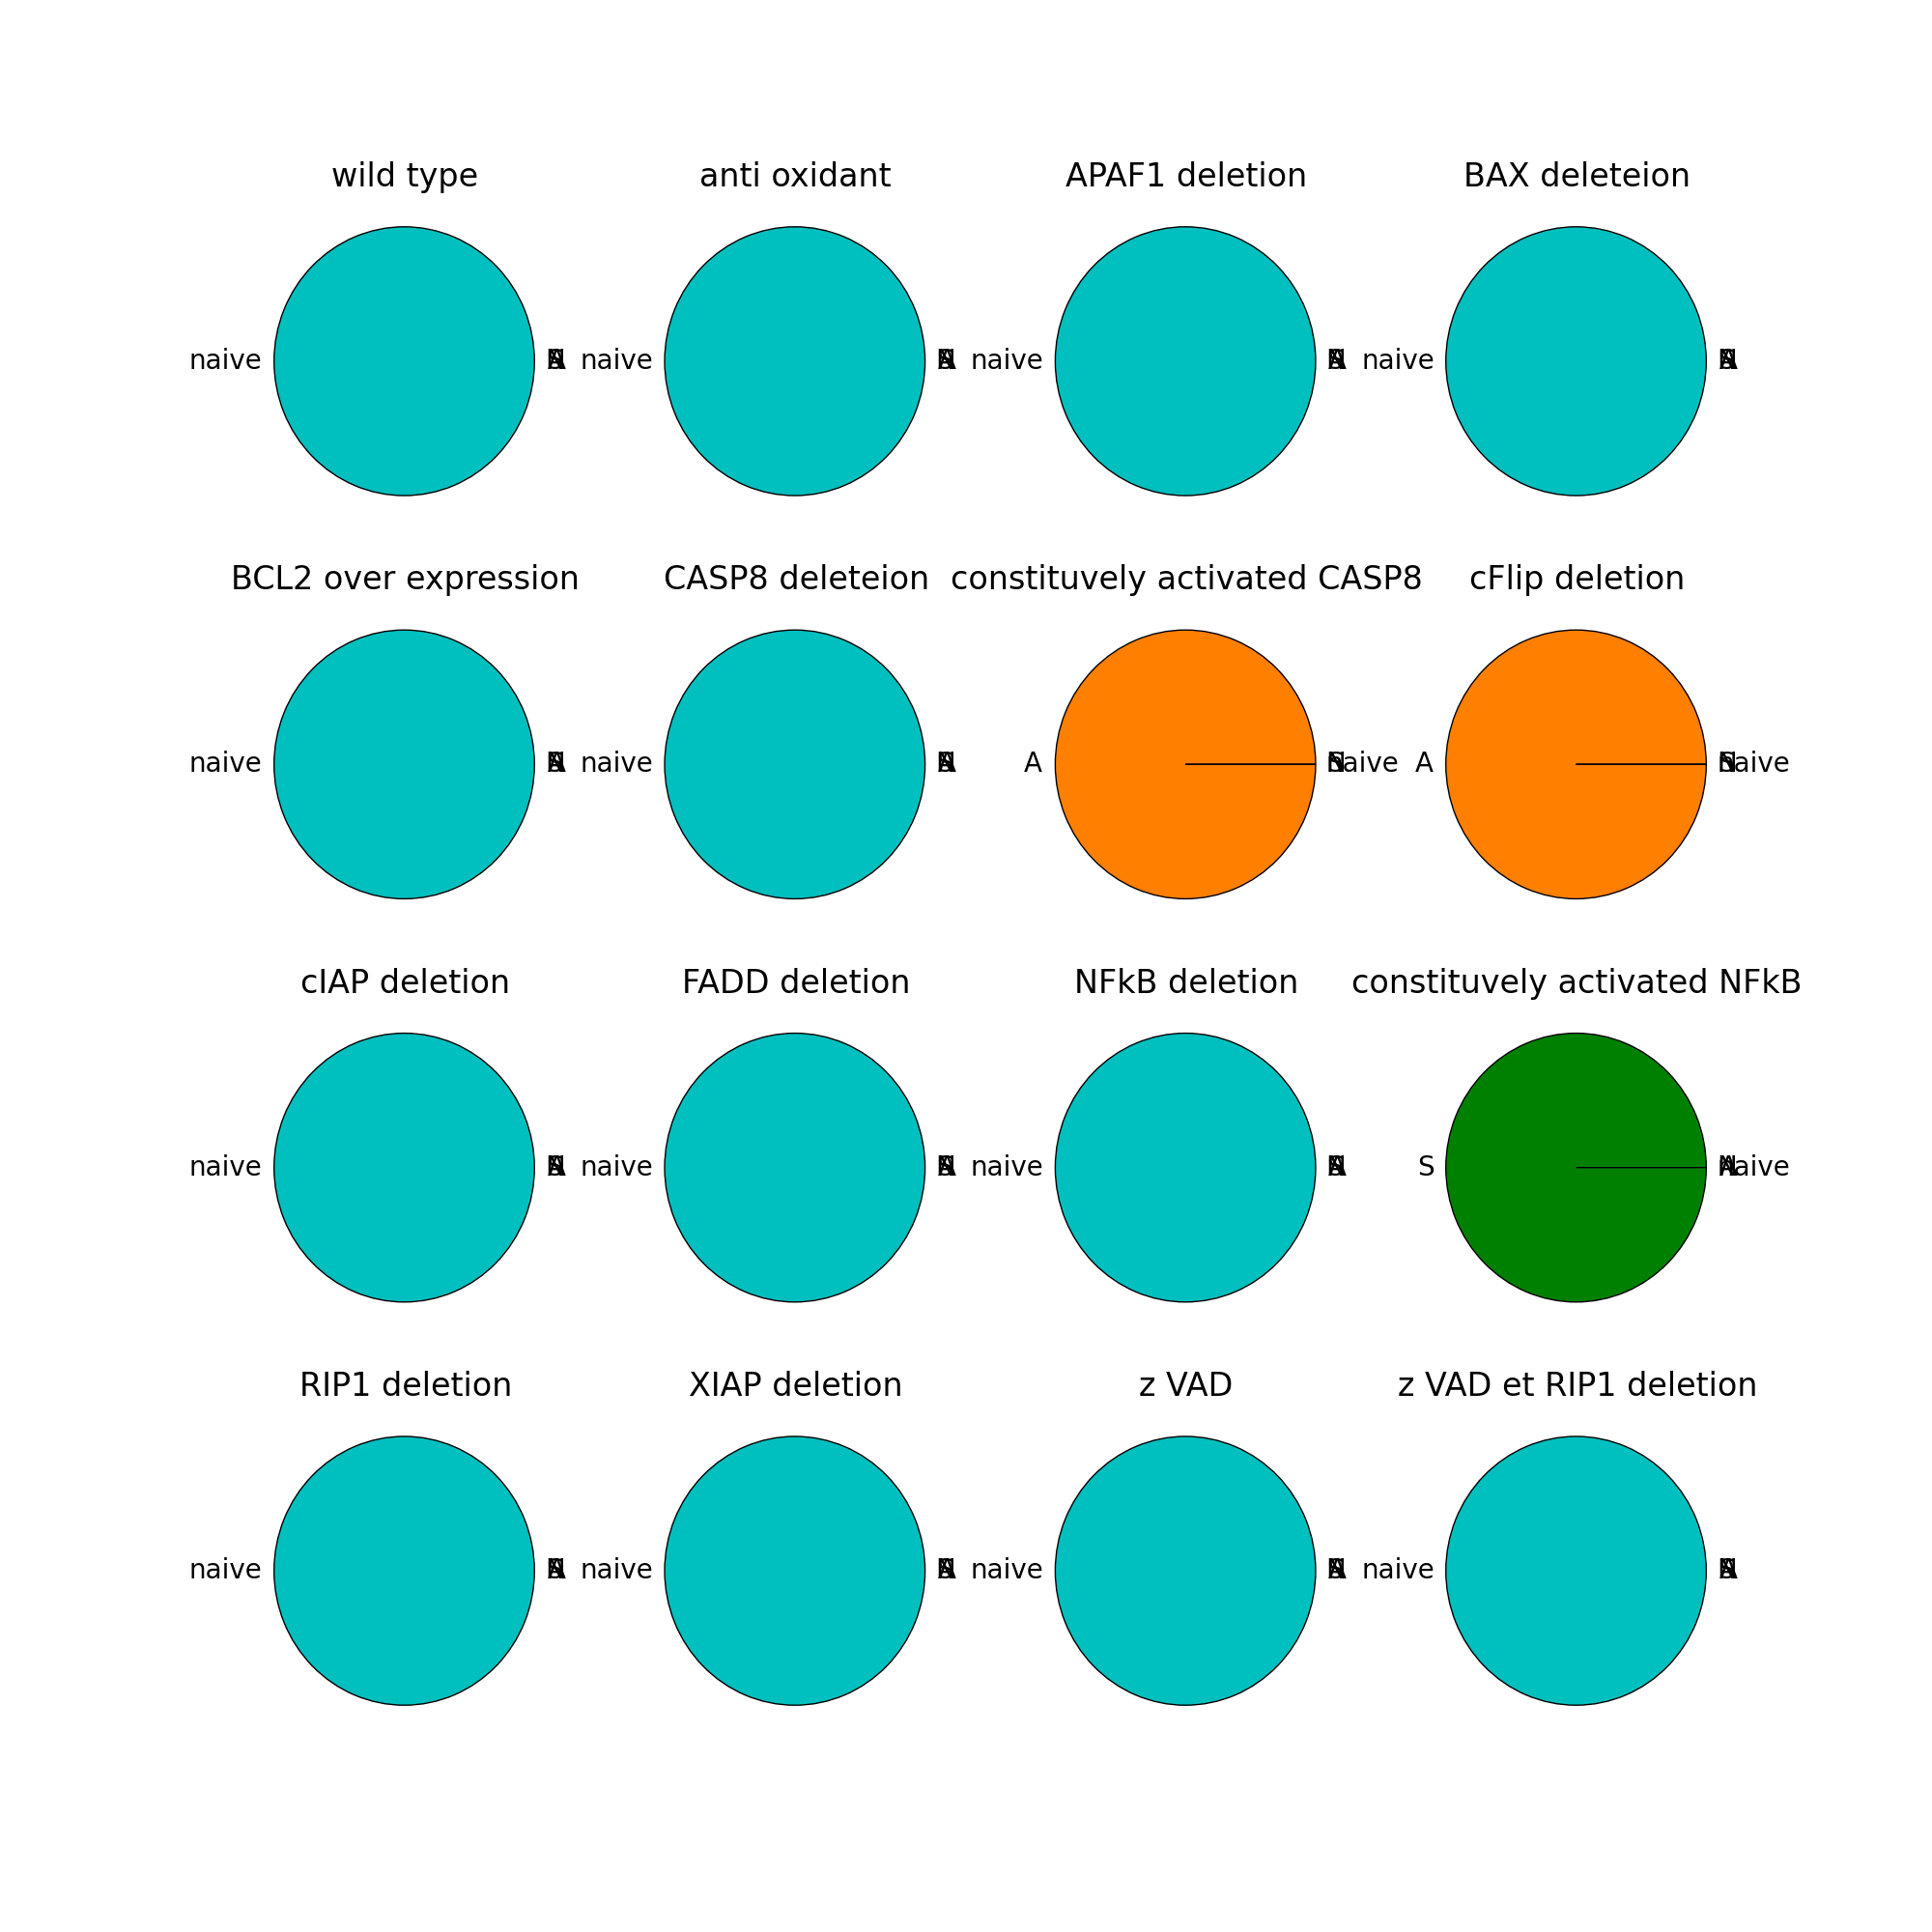
\includegraphics[scale=0.25]{tnf0_fas0}
        \caption{
            \label{tnf0_fas0}
            Résultat du choix du destin cellulaire sans l'activation des
            récepteurs \texttt{FAS} et \texttt{TNF}. En orange : mort par
            apoptose. En violet : mort par nécrose. En vert : survie. En cyan :
            choix indéterminé.
        }
    \end{center}
\end{figure}

\begin{figure}[position]
    \begin{center}
        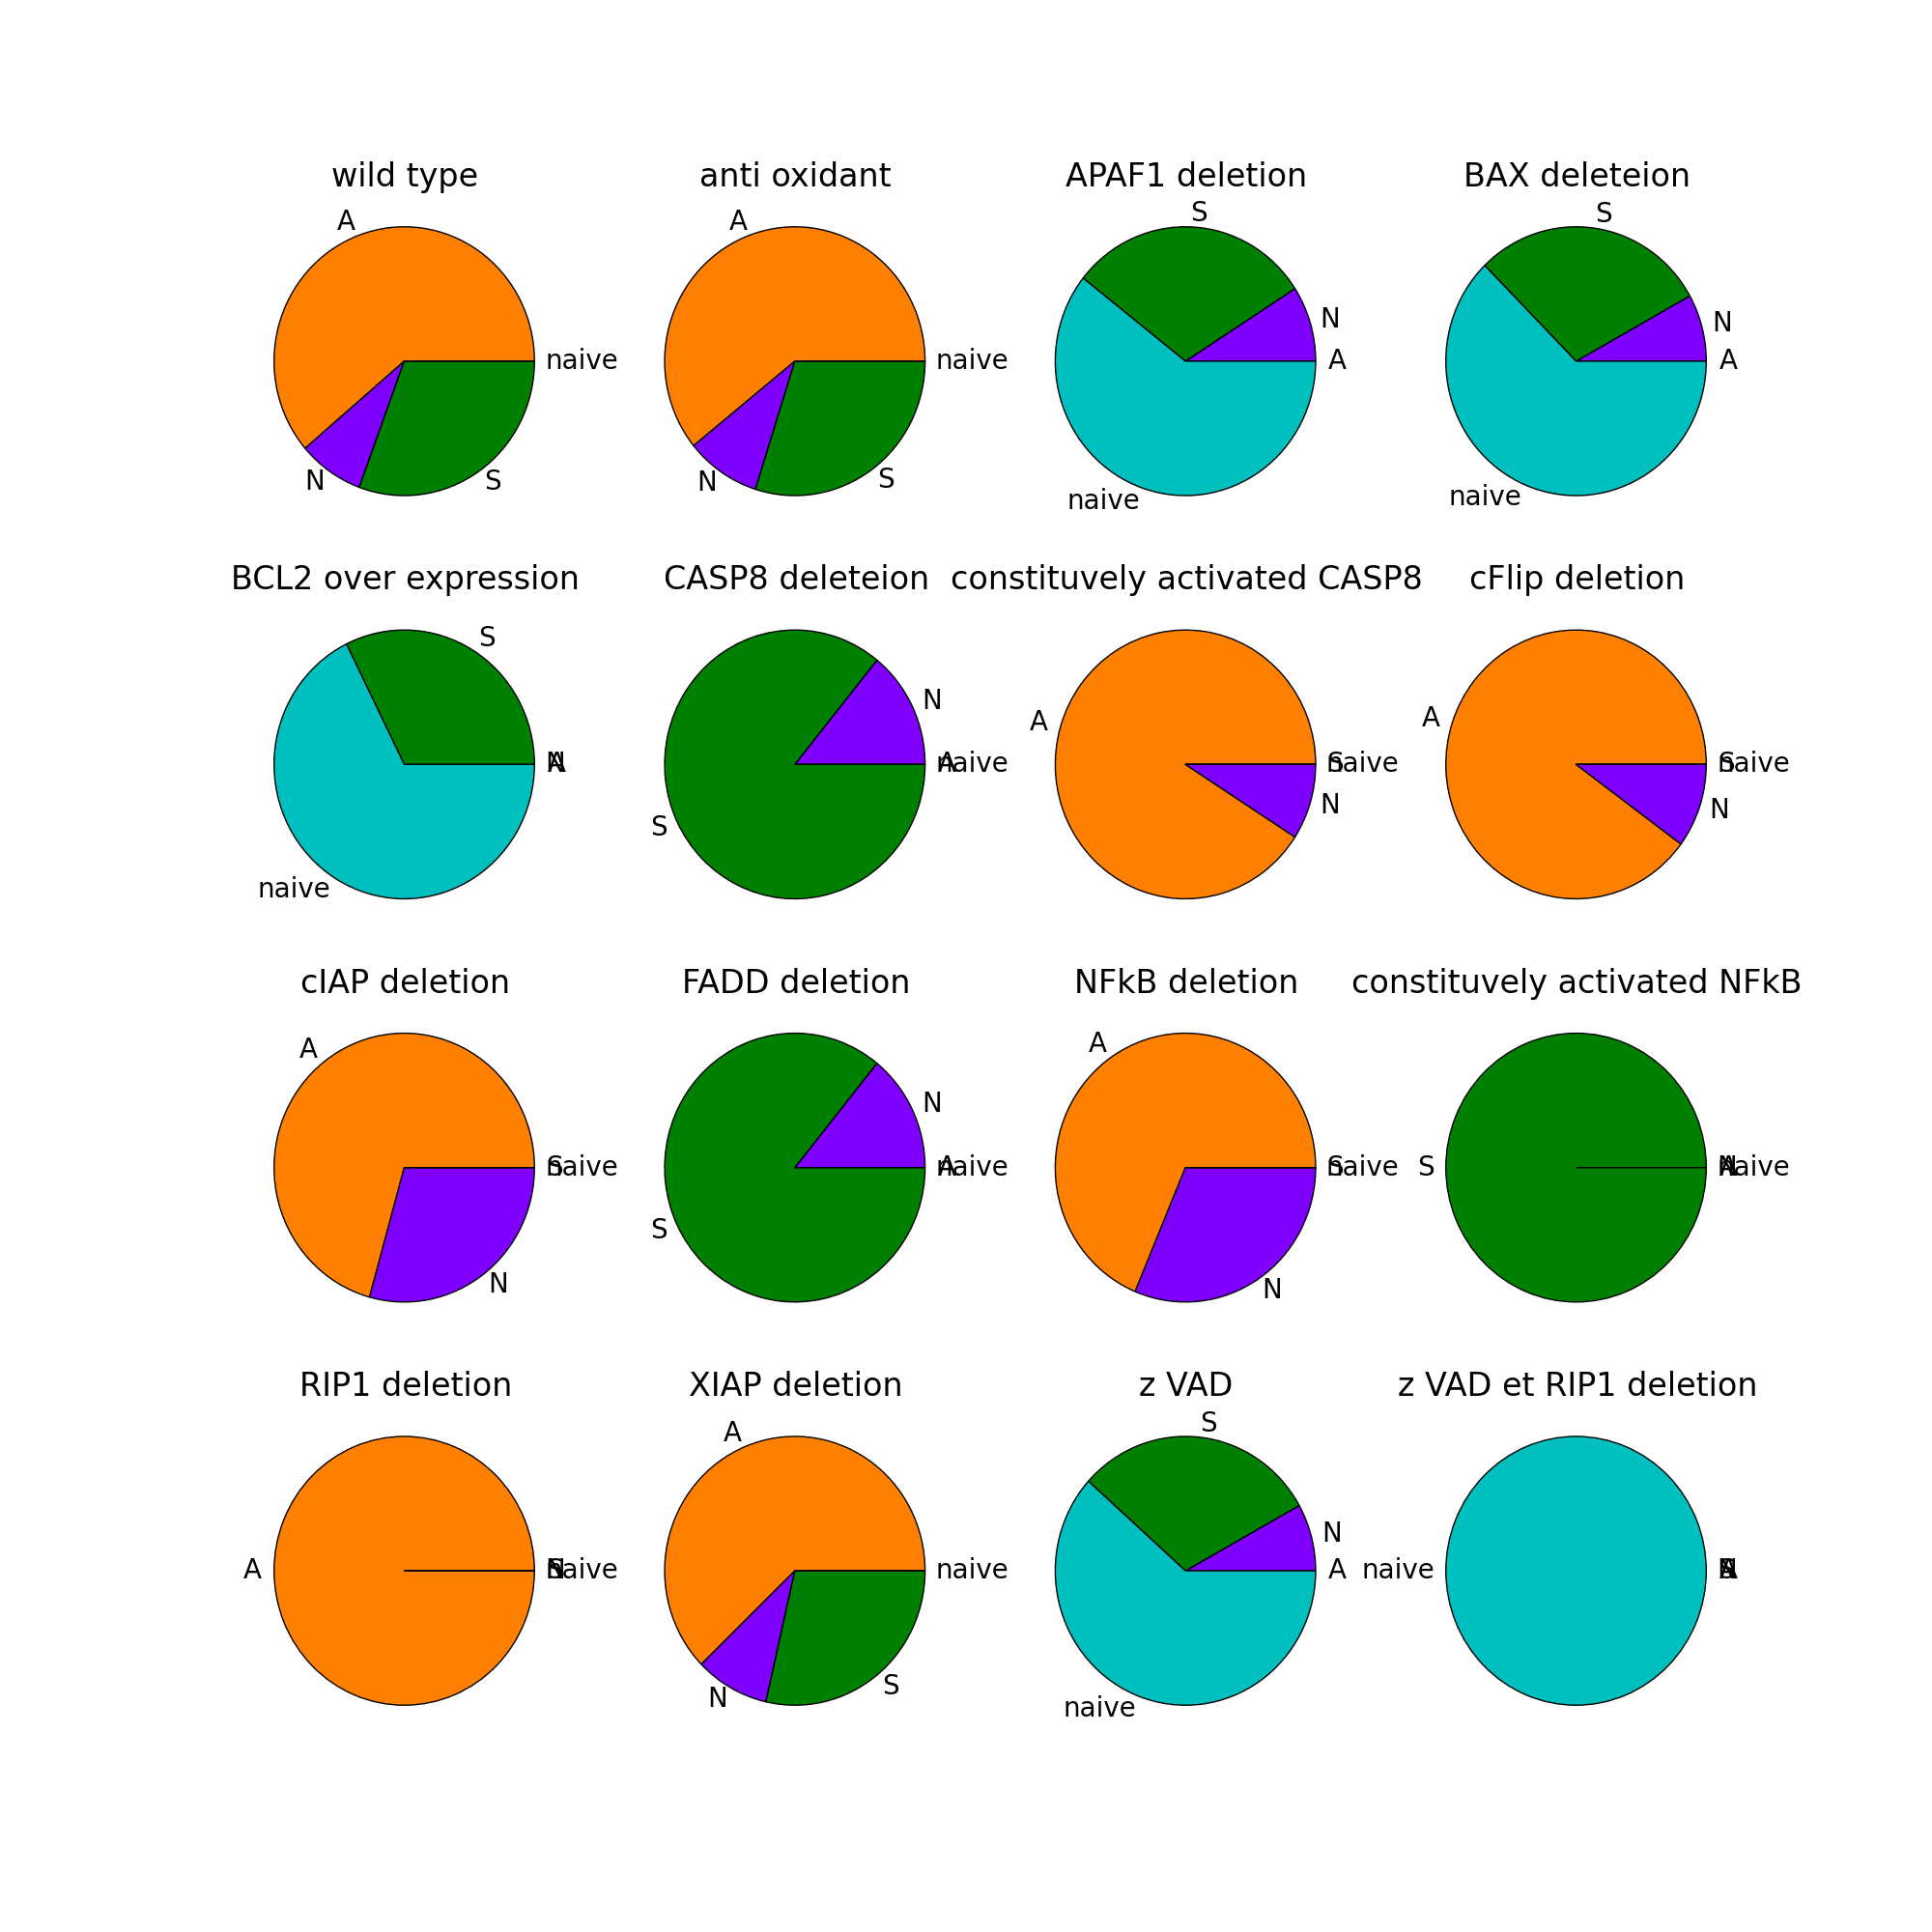
\includegraphics[scale=0.25]{tnf1_fas0}
        \caption{
            \label{tnf1_fas0}
            Résultat du choix du destin cellulaire sans l'activation du
            récepteur \texttt{FAS} et activation du \texttt{TNF}. En orange :
            mort par apoptose. En violet : mort par nécrose. En vert : survie.
            En cyan : choix indéterminé.
        }
    \end{center}
\end{figure}

\begin{figure}[position]
    \begin{center}
        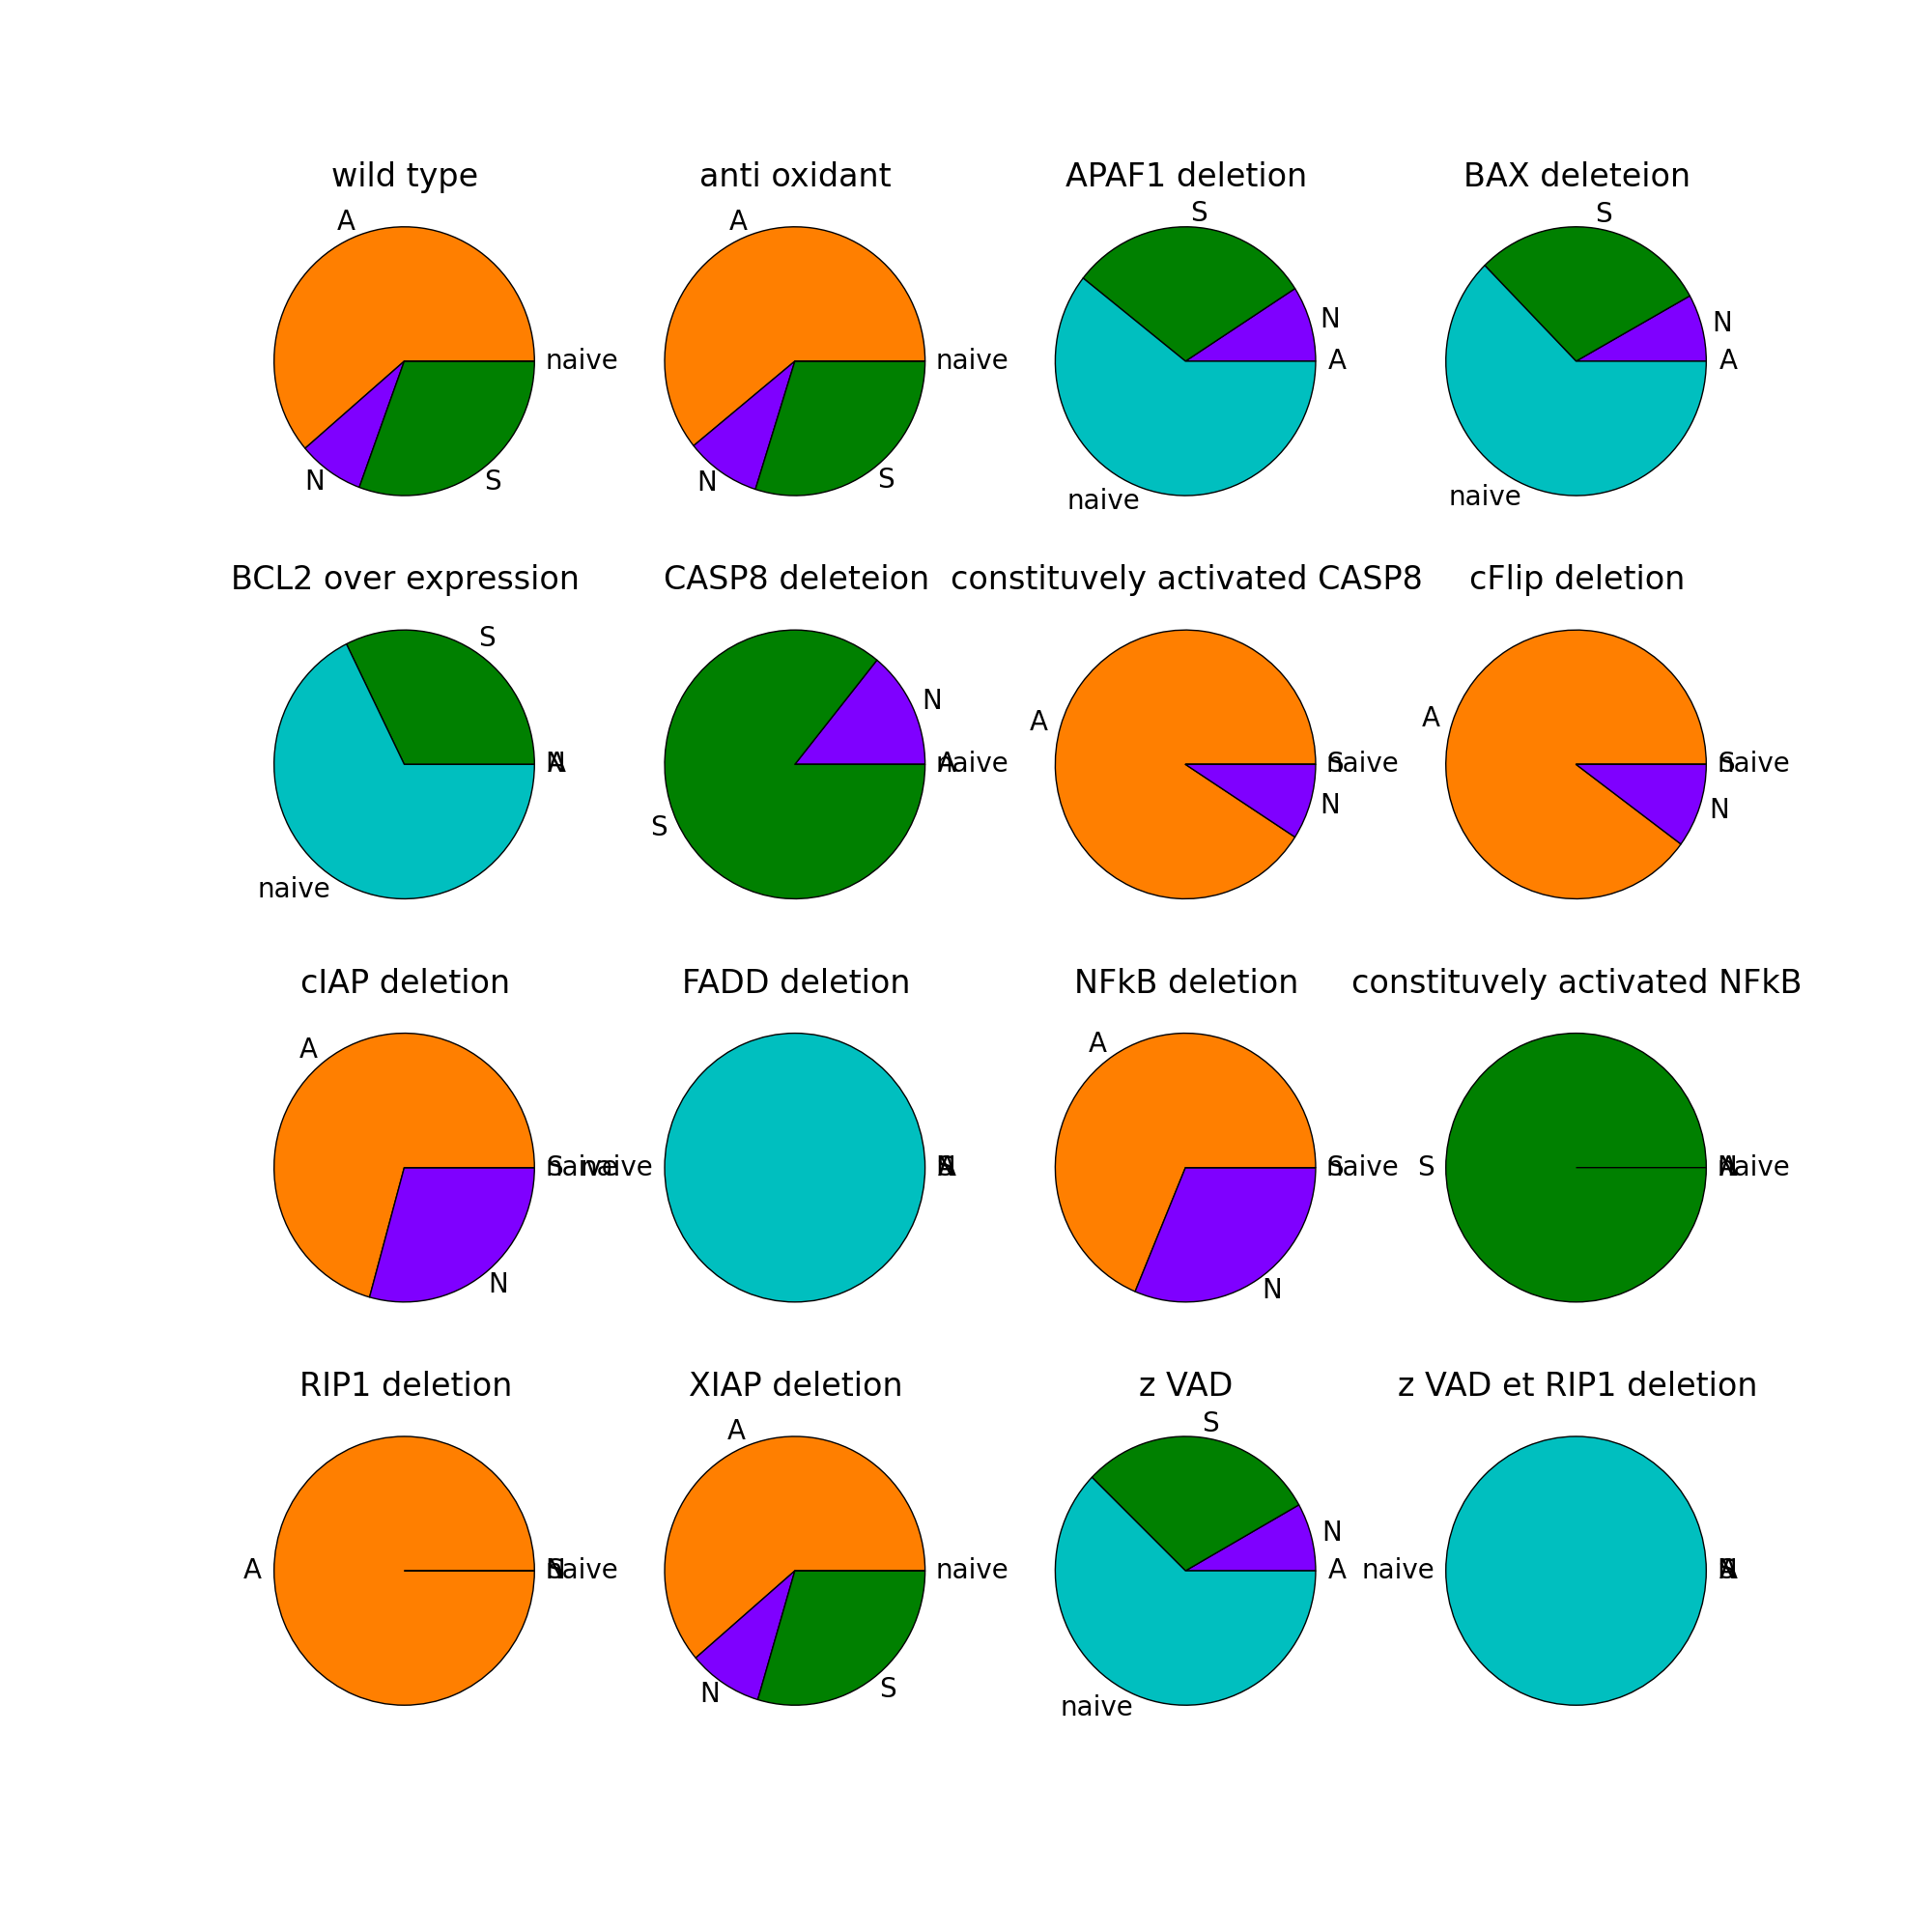
\includegraphics[scale=0.25]{tnf0_fas1}
        \caption{
            \label{tnf0_fas1}
            Résultat du choix du destin cellulaire sans l'activation du
            récepteur \texttt{TNF} et activation du \texttt{FAS}. En orange :
            mort par apoptose. En violet : mort par nécrose. En vert : survie.
            En cyan : choix indéterminé.
        }
    \end{center}
\end{figure}

\begin{figure}[position]
    \begin{center}
        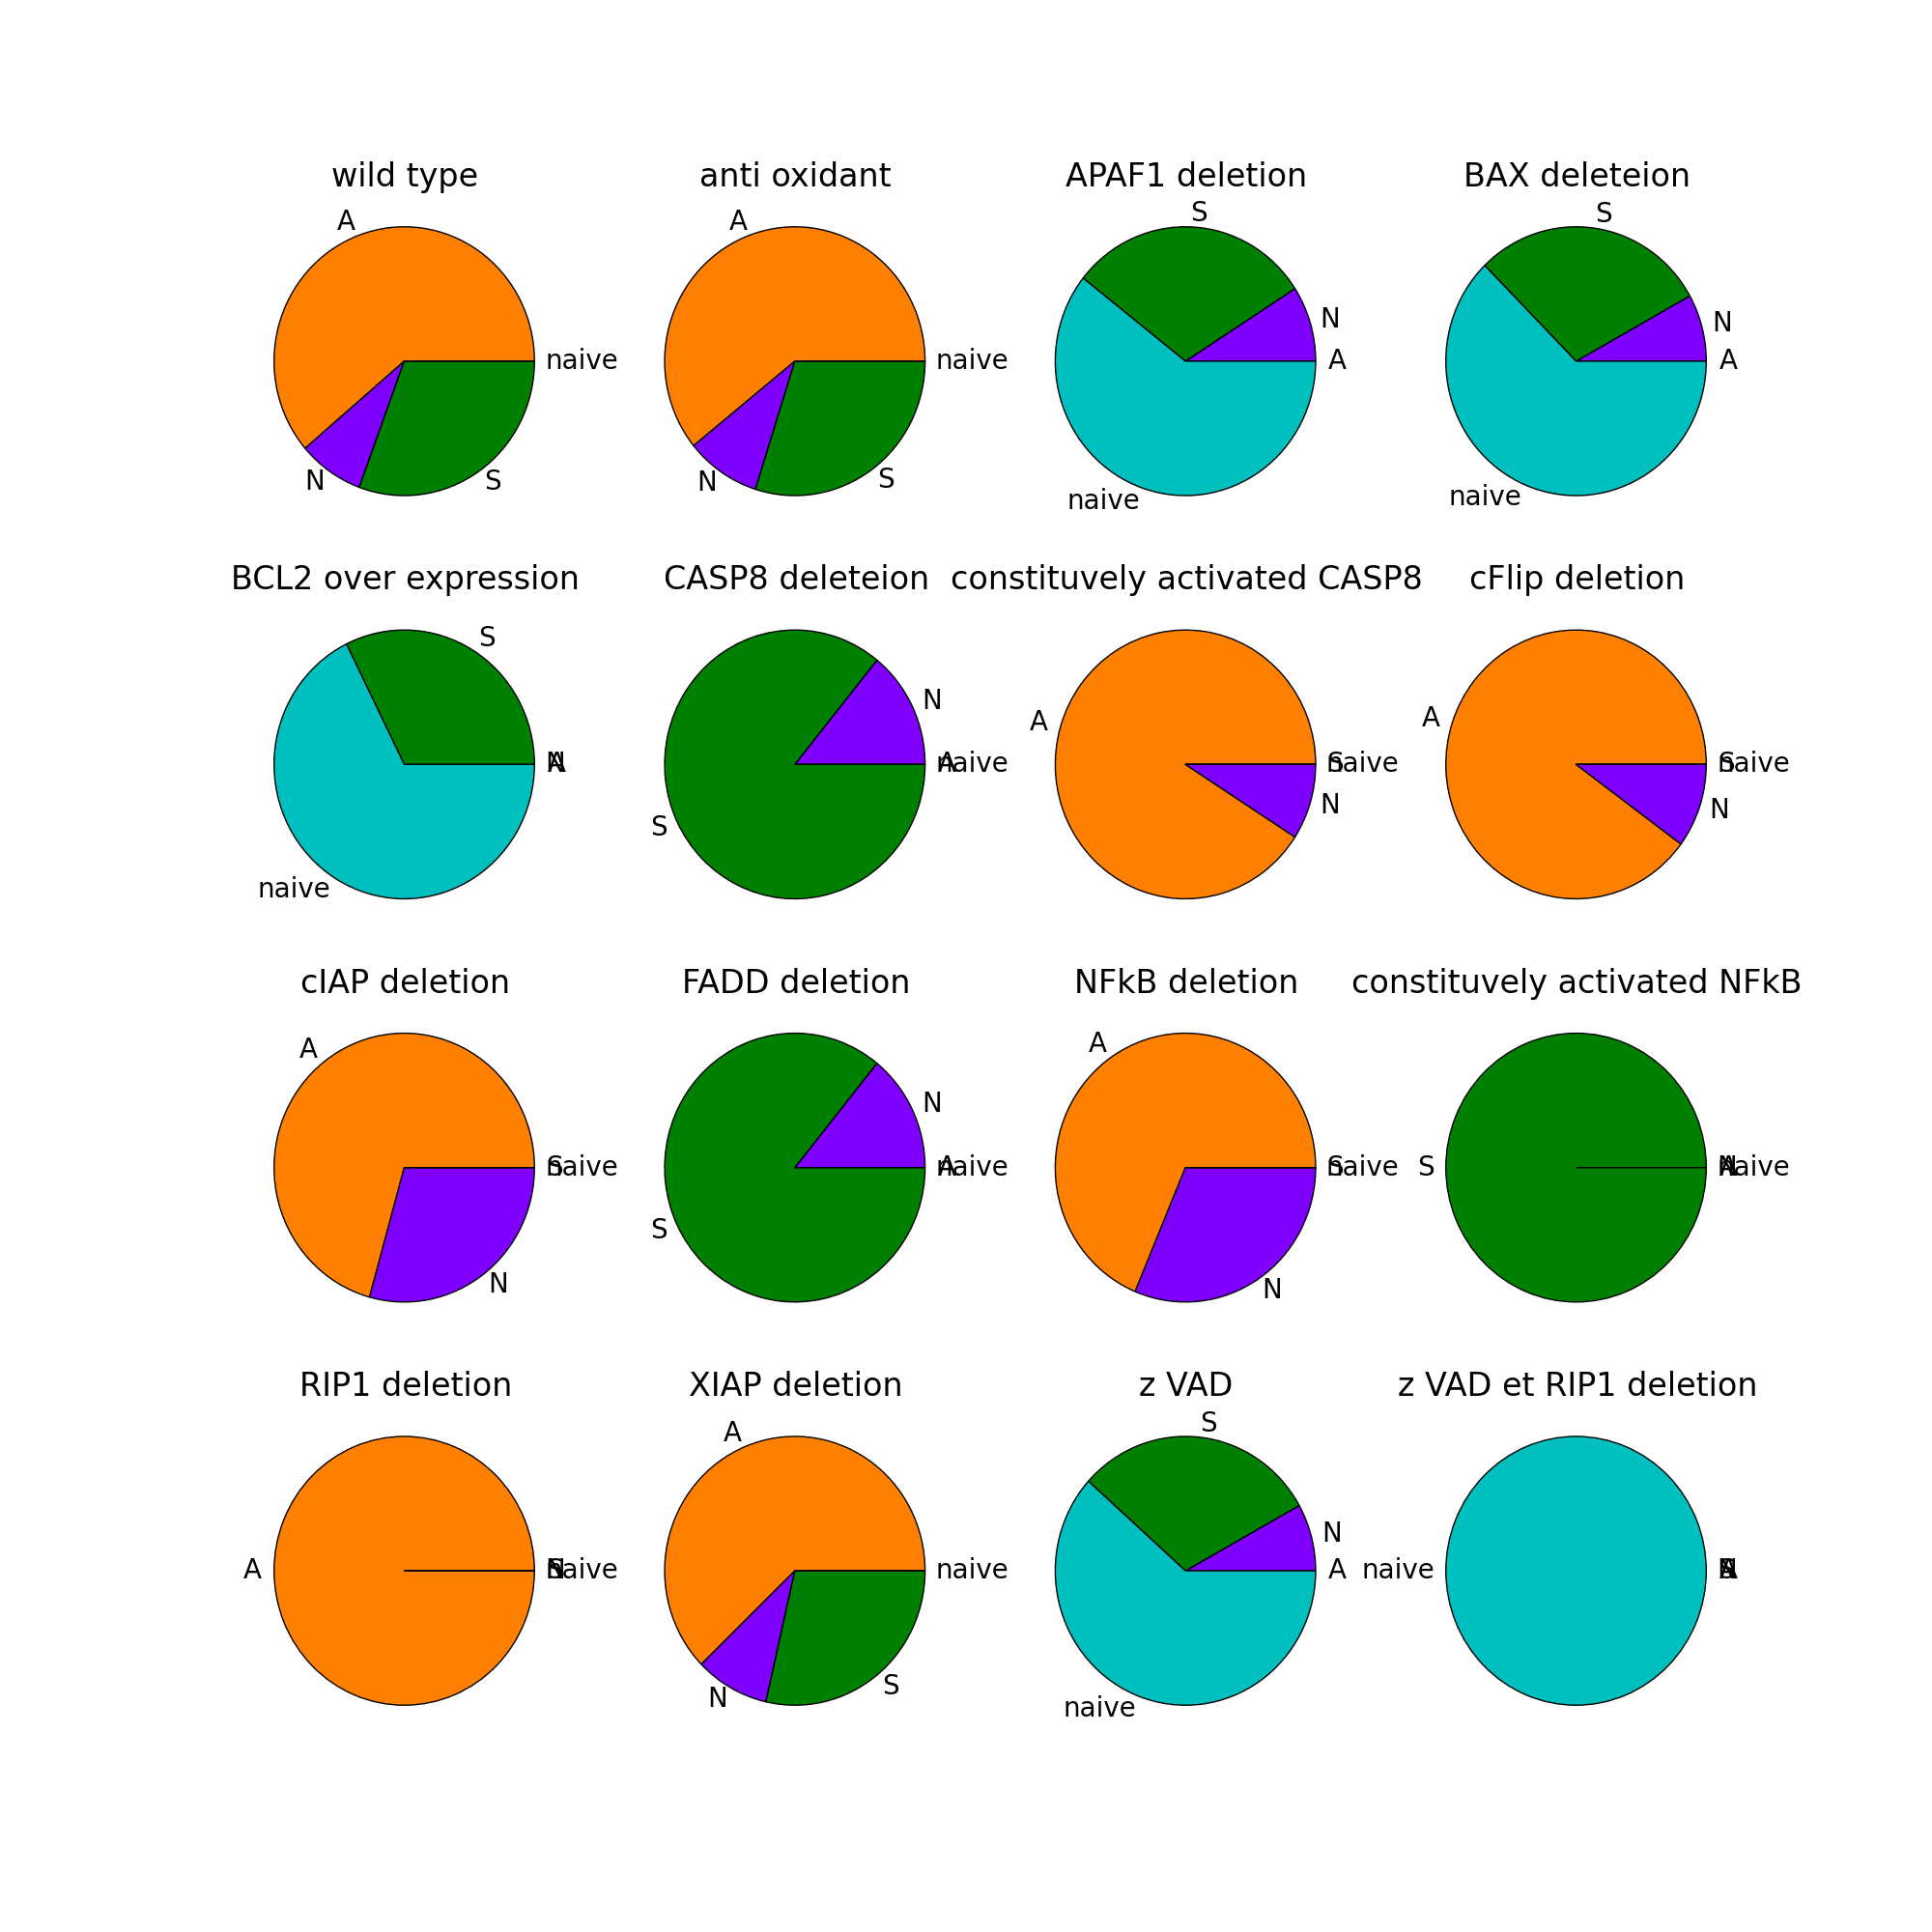
\includegraphics[scale=0.25]{tnf1_fas1}
        \caption{
            \label{tnf1_fas1}
            Résultat du choix du destin cellulaire avec l'activation des
            récepteurs \texttt{TNF} et \texttt{FAS}. En orange : mort par
            apoptose. En violet : mort par nécrose. En vert : survie. En cyan :
            choix indéterminé.
        }
    \end{center}
\end{figure}

Des tests plus approfondis n'ont pas pu être fait car l'intégration de la mort
au sein de la population cellulaire n'était pas totalement gérée.

\subsection{Aperçu de la dynamique du cycle cellulaire}
La machine du cycle cellulaire est totalement déterministe. Cela facilite la
méthode d'obtention des résultats. De plus il n'y a qu'une seule entrée qui
sert normalement à réarmer la dynamique du réseau booléen. On ne prend donc pas
ce noeud en compte et on le laisse à zéro. Les paramètres $A_g$, $A_r$ et $T_d$
ont été fixé pour la simulation. On a $A_g = 1, A_r = -1, T_d = 1$.

Comme ce modèle est déterministe et que la taille du réseau n'est que 11 (on
retire le noeud \texttt{Cell Size} pour cette simulation), la convergence de
tous les états possibles \footnote{Avec 11 noeuds à 2 états possibles, il y a
$2^{11} = 2048$ états possibles} est calculée dans cette simulation. On
récupère alors la liste des états finaux ainsi que le nombre d'états initiaux
menant à ceux-ci. Cette liste est représentée dans le tableau
\ref{table_yeast}.

\begin{center}
    \begin{table}
        \caption{
            \label{table_yeast}
            Liste des bassins d'attractions avec le nombre d'états étant
            dedans. Un 1 indique que le noeud est activé. Un 0 qu'il est
            désactivé.
        }
        \small
        \begin{tabular}{r | c c c c c c c c c c c}
            Nombre & Cln3 & MBF & SBF & Cln1,2 & Cdh1 & Swi5 & Cdc20 & Clb5,6 &
            Sic1 & Clb1,2 & Mcm1 \\
            \hline
            7       & 0 & 0 & 0 & 0 & 0 & 0 & 0 & 0 & 0 & 0 & 0 \\
            151     & 0 & 0 & 1 & 1 & 0 & 0 & 0 & 0 & 0 & 0 & 0 \\
            1       & 0 & 0 & 0 & 0 & 1 & 0 & 0 & 0 & 0 & 0 & 0 \\
            9       & 0 & 0 & 0 & 0 & 0 & 0 & 0 & 0 & 1 & 0 & 0 \\
            1764    & 0 & 0 & 0 & 0 & 1 & 0 & 0 & 0 & 1 & 0 & 0 \\
            7       & 0 & 1 & 0 & 0 & 0 & 0 & 0 & 0 & 1 & 0 & 0 \\
            109     & 0 & 1 & 0 & 0 & 1 & 0 & 0 & 0 & 1 & 0 & 0 \\
        \end{tabular}
        \normalsize
    \end{table}
\end{center}

Un des bassins est en majorité par rapport aux autres. On remarque également
que lorsqu'on active le noeud d'entrée \texttt{Cell Size}, on reste dans ce
bassin et le résultat converge à nouveau vers ce dernier résultat. On peut
alors voir le chemin de cet état initial jusqu'au point de convergence sur le
tableau \ref{cycle_path}.

\begin{center}
    \begin{table}
        \caption{
            \label{cycle_path}
            Évolution temporelle du chemin bouclé avec réarmement par le noeud
            d'entrée.
        }
        \small
        \begin{tabular}{c c c c c c c c c c c c}
            Cell Size & Cln3 & MBF & SBF & Cln1,2 & Cdh1 & Swi5 & Cdc20 &
            Clb5,6 & Sic1 & Clb1,2 & Mcm1 \\
            \hline
            0 & 0 & 0 & 0 & 0 & 1 & 0 & 0 & 0 & 1 & 0 & 0 \\
            1 & 0 & 0 & 0 & 0 & 1 & 0 & 0 & 0 & 1 & 0 & 0 \\
            0 & 1 & 0 & 0 & 0 & 1 & 0 & 0 & 0 & 1 & 0 & 0 \\
            0 & 0 & 1 & 1 & 0 & 1 & 0 & 0 & 0 & 1 & 0 & 0 \\
            0 & 0 & 1 & 1 & 1 & 1 & 0 & 0 & 0 & 1 & 0 & 0 \\
            0 & 0 & 1 & 1 & 1 & 0 & 0 & 0 & 0 & 0 & 0 & 0 \\
            0 & 0 & 1 & 1 & 1 & 0 & 0 & 0 & 1 & 0 & 0 & 0 \\
            0 & 0 & 1 & 1 & 1 & 0 & 0 & 0 & 1 & 0 & 1 & 1 \\
            0 & 0 & 0 & 0 & 1 & 0 & 0 & 1 & 1 & 0 & 1 & 1 \\
            0 & 0 & 0 & 0 & 0 & 0 & 1 & 1 & 0 & 0 & 1 & 1 \\
            0 & 0 & 0 & 0 & 0 & 0 & 1 & 1 & 0 & 1 & 1 & 1 \\
            0 & 0 & 0 & 0 & 0 & 0 & 1 & 1 & 0 & 1 & 0 & 1 \\
            0 & 0 & 0 & 0 & 0 & 1 & 1 & 1 & 0 & 1 & 0 & 0 \\
            0 & 0 & 0 & 0 & 0 & 1 & 1 & 0 & 0 & 1 & 0 & 0 \\
            0 & 0 & 0 & 0 & 0 & 1 & 0 & 0 & 0 & 1 & 0 & 0 \\
        \end{tabular}
        \normalsize
    \end{table}
\end{center}

En ayant testé avec différentes valeurs des paramètres, on retrouve les même
sept points de convergence avec une majorité pour le même tant qu'on suit les
conditions dites plus haut.

La machine choisissant entre la différentiation et le renouvellement est
également disponible et testée \footnote{Voir le dossier
\texttt{examples/decision\_gata1}}. Cette machine est entièrement déterministe
et les résultats attendus sont atteints. C'est-à-dire que tant que la présence
d'\texttt{EPO} n'est pas continu pendant un certain temps, le noeud
\texttt{GATA-1} n'est pas activé. Si le seuil de temps est dépassé, alors
\texttt{GATA-1} est activé et le reste tant qu'il n'y a pas une
réinitialisation demandée par l'utilisateur.

\subsection{Synchronisation de l'oscillateur booléen}
\begin{figure}[position]
    \begin{center}
        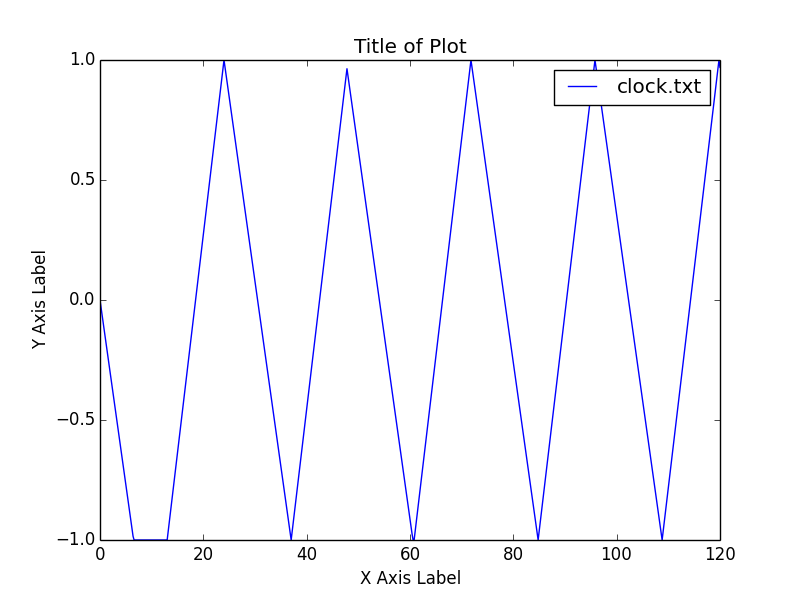
\includegraphics[scale=0.4]{clock}
        \caption{
            \label{result_clock}
            Signal de l'horloge interne d'une cellule basée sur le signal carré
            de son réseau booléen intracellulaire. Les abscisses sont des
            heures et les ordonnées sont un taux d'avancement de l'horloge
            entre $1$ et $-1$.
        }
    \end{center}
\end{figure}

La figure \ref{result_clock} montre l'interprétation de la cellule en fonction
de sa propre machine interne servant d'oscillateur. Pour l'instant, le signal
carré n'est transformé qu'en simple signal triangulaire par intégration. Ce
signal est voulu pour travailler sur la synchronisation de la population autour
d'un signal simple. Ces travaux n'ont pas totalement aboutis. Il y a tout de
même quelques résultats visibles sur la figure \ref{result_clock_sync_loc}. La
figure \ref{result_clock_sync} représente le graphique de synchronisation de la
simulation correspondante.

\begin{figure}[position]
    \begin{center}
        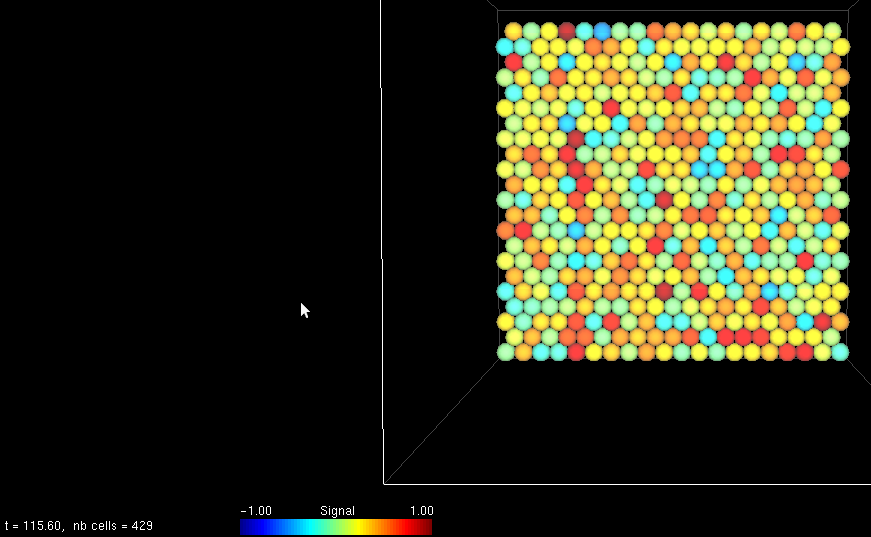
\includegraphics[scale=0.3]{result_clock_sync_loc}
        \caption{
            \label{result_clock_sync_loc}
            Représentation de la population après 115 heures dans la
            simulation. Les couleurs des cellules représentent le signal
            visualisé (l'horloge ici). On peut voir que les horloges sont
            synchronisés localement et qu'il y a un effet de dissipation de la
            synchronisation.
        }
    \end{center}
\end{figure}

\begin{figure}[position]
    \begin{center}
        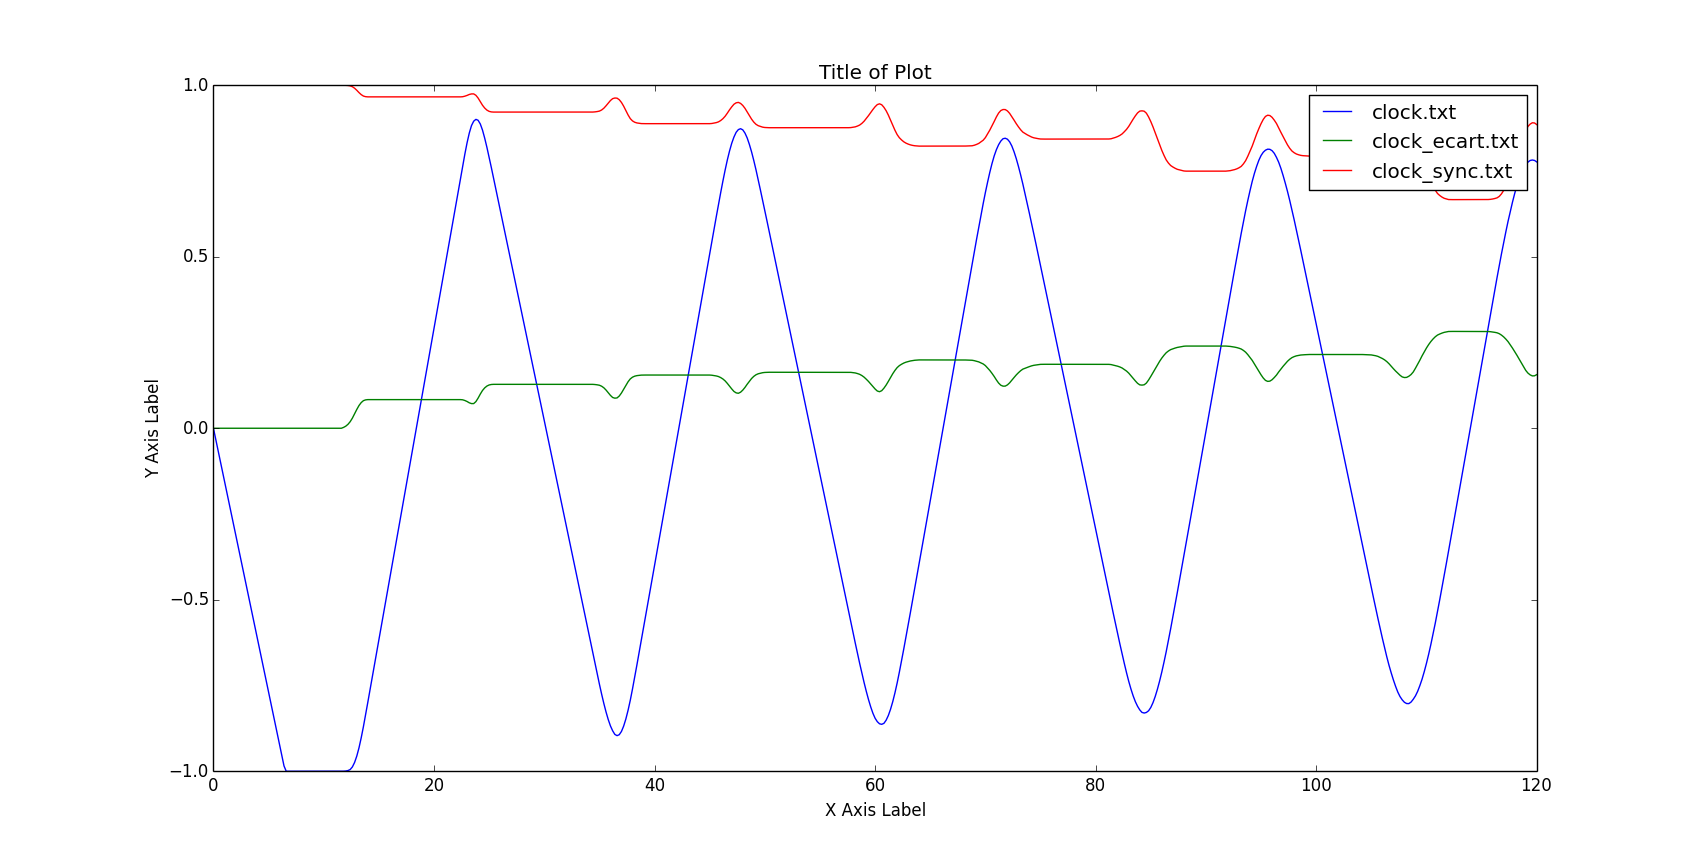
\includegraphics[scale=0.35]{result_clock_sync}
        \caption{
            \label{result_clock_sync}
            Représentation de la moyenne, l'écart type et du taux de
            synchronisation du signal de l'horloge en fonction de l'heure passé
            dans la simulation. En bleu : moyenne sur toutes les cellules du
            signal de l'horloge. En vert : écart type des horloges de chaque
            cellule. En rouge : taux de synchronisation (1 correspond à une
            synchronisation parfaite et 0 à une désynchronisation totale).
        }
    \end{center}
\end{figure}

\newpage
\section{Discussion et conclusion}
L'implémentation de la bibliothèque fournie permet de modéliser facilement
différents type de réseaux booléens allant des plus simples utilisant des
règles booléennes explicitement écrites ou allant à des plus complexe avec une
représentation matricielle dont les coefficients peuvent être des structures de
données complexe. Les différents tests effectués sont concluants : nous avons
pu implémenter en parallèle plusieurs modèles de la littérature. \\

Les résultats des simulations de la machine de choix du destin cellulaire
correspondent à ceux retrouvés dans la littérature \cite{calzone2010}. Excepté
pour la mutation \texttt{z-VAD}, qui désactive la protéine \texttt{CASP3} ainsi
que le noeud correspondant. Cette erreur de reproduction apparaissait aussi
lorsque le système était modélisé par des règles booléennes. Ces règles qui
étaient alors les même que la littérature. Nous considérons quand même le test
comme valide.

On remarque que l'activation, soit du \texttt{TNF}, soit du \texttt{FAS}, ou
des deux produit un résultat assez proche. Les résultats obtenus sont tout de
même assez proche des résultats attendus autant pour la cellule de base que
pour les mutantes. Lorsqu'un des facteurs de mort cellulaire est actif, le taux
de mort par apoptose ou par nécrose est bien augmenté et est même en majorité
dans la plupart des cas. De plus, on voit également que les cas de mutations
triviaux sont bons. Par exemple, lorsque le \texttt{CASP8} est supprimé, il n'y
a plus de mort par apoptose. \\

La machine du cycle cellulaire montre une certaine boucle dans sa simulation et
une fois qu'elle a convergé, il est possible de réarmer la machine juste en
activant un noeud en fonction de la taille de la cellule en question. Cette
boucle peut être utilisée pour représenter le cycle cellulaire et permet donc
de retrouver les 4 différentes phases de ce cycle. \\

L'horloge et sa synchronisation est à revoir. En effet, le signal utilisé n'est
qu'un simple signal carré qui ne ressemble donc pas exactement aux signaux des
horloges circadiennes. De plus, la synchronisation s'atténue un peu au cours du
temps comme le montre les figures (\ref{result_clock_sync_loc},
\ref{result_clock_sync}). La synchronisation peut être améliorée en modifiant
la valeur du coefficient de force de couplage utilisé ainsi  qu'en réduisant
la constante d'écart stochastique utilisée dans l'avancement de l'oscillateur
booléen. On remarque également que les effets de synchronisation se font
souvent localement. En effet, comme une cellule ne peut communiquer qu'avec ses
voisines, l'effet de synchronisation doit se déplacer le long de toute la
population pour faire effet. Ce déplacement prend un certain temps et on voit
alors apparaître des ``vague'' de transmissions d'informations. \\

L'implémentation des réseaux est faite, il reste, toutefois, à les configurer
et à les corriger sur certains points pour produire le plus fidèlement les
résultats voulus. En effet, la mort cellulaire n'est pas totalement gérée,
ainsi que le choix entre la différentiation et le renouvellement. Les horloges
ne sont pas non plus totalement synchronisées entre elles. Aussi, il serait
intéressant de définir une machine choisissant quelle mutation prendre pour la
cellule et quand.

Ce modèle cellulaire n'est pas complet mais il peut être comblé facilement en
rajoutant des aspects internes en utilisant d'autres réseaux booléens.

\newpage
\bibliographystyle{unsrt}
\bibliography{main}
\addcontentsline{toc}{section}{Références}
\end{document}
